\documentclass[t,14pt,aspectratio=169]{beamer}
\usepackage{ep-dark}   % JHU/WSE style for use on Lightboard
\usepackage{graphicx}  % for inclusion of graphics
\usepackage{amsmath}   % good for additional math
\usepackage{amsthm}    % theorems, definitions, etc

%\usetheme{CambridgeUS}

%% Oh yes. TIKZ pictures / graphs
%% -------------------------------------
\usepackage{tikz}
\usepackage{pgfplots}
\usepackage{tikz-3dplot}
\usepackage{tkz-euclide}
\usetikzlibrary{calc,fadings,decorations.pathreplacing,shadings,intersections,backgrounds}

%% This is when making tikz plots
%% -------------------------------------
\pgfplotsset{rdstyle/.style={%
        width=8cm,
        ylabel={y},
        xlabel={x},
        xmin=-2,xmax=3,
        xtick={-2,-1,...,3}}}
%% -------------------------------------

%% Axis rotator for arrows rotating around vector
%% -------------------------------------
\newcommand{\AxisRotator}[1][rotate=0]{%
    \tikz [x=0.25cm,y=0.60cm,line width=.2ex,-stealth,#1] \draw (0,0) arc (-150:150:1 and 1);%
}
%% -------------------------------------

%% Animations
%% -------------------------------------
\usepackage{animate}

%% This is the UT logo in the top right.
%% -------------------------------------
\logo {
\begin{tikzpicture}[overlay,remember picture]
\coordinate (A) at (-4.3,8.0);
\node[left=0.2cm] at (current page.27){
    
\includegraphics[width=3cm]{Figures/General/UT_WBMW_Rot_RGB_01.png}
    %
\includegraphics[width=3cm]{Figures/General/UT_WBMW_Weiss_1C_tr.png}
};
\node[text=Karminrot] at (A) {\tiny Introduction to Geophysics};
\end{tikzpicture}
}
%% -------------------------------------

%% -------------------------------------
%% Customized Environments

%%Empty column left, 1/3 filled right
%%Arguments is frametitle
\newenvironment{PointThree}[1]
{  \frametitle{#1}
  \begin{columns}[c, onlytextwidth]%EVEN SPECIFYING THE c OPTION
    \begin{column}{.6\textwidth}%
        \setlength{\partopsep}{0pt}%AND EVEN REMOVING EXTRA itemize SPACE
        % Keep this empty
    \end{column}%
    \begin{column}{.35\textwidth}
}
{
    \end{column}%
  \end{columns}
}
\newenvironment{PointSix}[1]
{  \frametitle{#1}
  \begin{columns}[c, onlytextwidth]%EVEN SPECIFYING THE c OPTION
    \begin{column}{.35\textwidth}%
        \setlength{\partopsep}{0pt}%AND EVEN REMOVING EXTRA itemize SPACE
        % Keep this empty
    \end{column}%
    \begin{column}{.6\textwidth}
}
{
    \end{column}%
  \end{columns}
}

%Input frame title and content left.
\newenvironment{ThreeCols}[2]
{
  \frametitle{#1}
  \begin{columns}[c, onlytextwidth]
    \begin{column}{.32\textwidth}%
        \setlength{\partopsep}{0pt}%AND EVEN REMOVING EXTRA itemize SPACE
        #2
    \end{column}%
    \begin{column}{.32\textwidth}
      %empty
    \end{column}%
    \begin{column}{.32\textwidth}

}
{
    \end{column}%
  \end{columns}
}
%% -------------------------------------




\title{Introduction to Geophysics}
\author{R. Drews}
\date{\today}


\begin{document}

% These commands create the first slide
% \coursename specifies the name of the course. No need to include the
% course number especially since they change from time to time
%
% \modulename is the name of this particular lesson

\coursename{Introduction to Geophysics}
\modulename{Gravity Method}
\titleframe

%
\begin{frame}
    % \small
    % \begin{PointSix}{How do we teach? }
    %     \begin{itemize}
    %         \item Video Lectures or Plenum (Tuesdays)
    %         \item Exercises \& 1-1-Interaction (Thursdays)
    %         \item Applied Exercises (Magnetics, Electrics, Seismics)
    %     \end{itemize}
    % \end{PointSix}
\end{frame}

\begin{frame}
  \begin{PointSix}{Introduction}
    \small
    \alert{Introduction to Geophysics}
    \begin{itemize}
      \item Who?
      \item What?
      \item How?
    \end{itemize}
  \end{PointSix}
  \end{frame}

\begin{frame}
    \begin{PointSix}{Who's teaching?}
        \small
        \begin{itemize}
            \item R. Drews (Prof. Geophysics at UT)
            \item P. Dietrich (Prof. Env./Eng.- Geophysics at UFZ, Leipzig)
            \item R. Ershadi (PhD Geophysics)
            \item A. Vinson (TA, MSc Geosciences)
            \item L. Naumann (TA, BSc Geosciences)
          \end{itemize}
    \end{PointSix}
\end{frame}

\begin{frame}
    \begin{PointSix}{Who's teaching?}
        \alert{Introduction to Geophysics - R. Drews}
        \small Prof. for Geophysics since 2022
      \end{PointSix}
\end{frame}

\begin{frame}
    \begin{PointSix}{Who's teaching?}
        \alert{Introduction to Geophysics - R. Drews}
        \small Prof. for Geophysics since 2022
        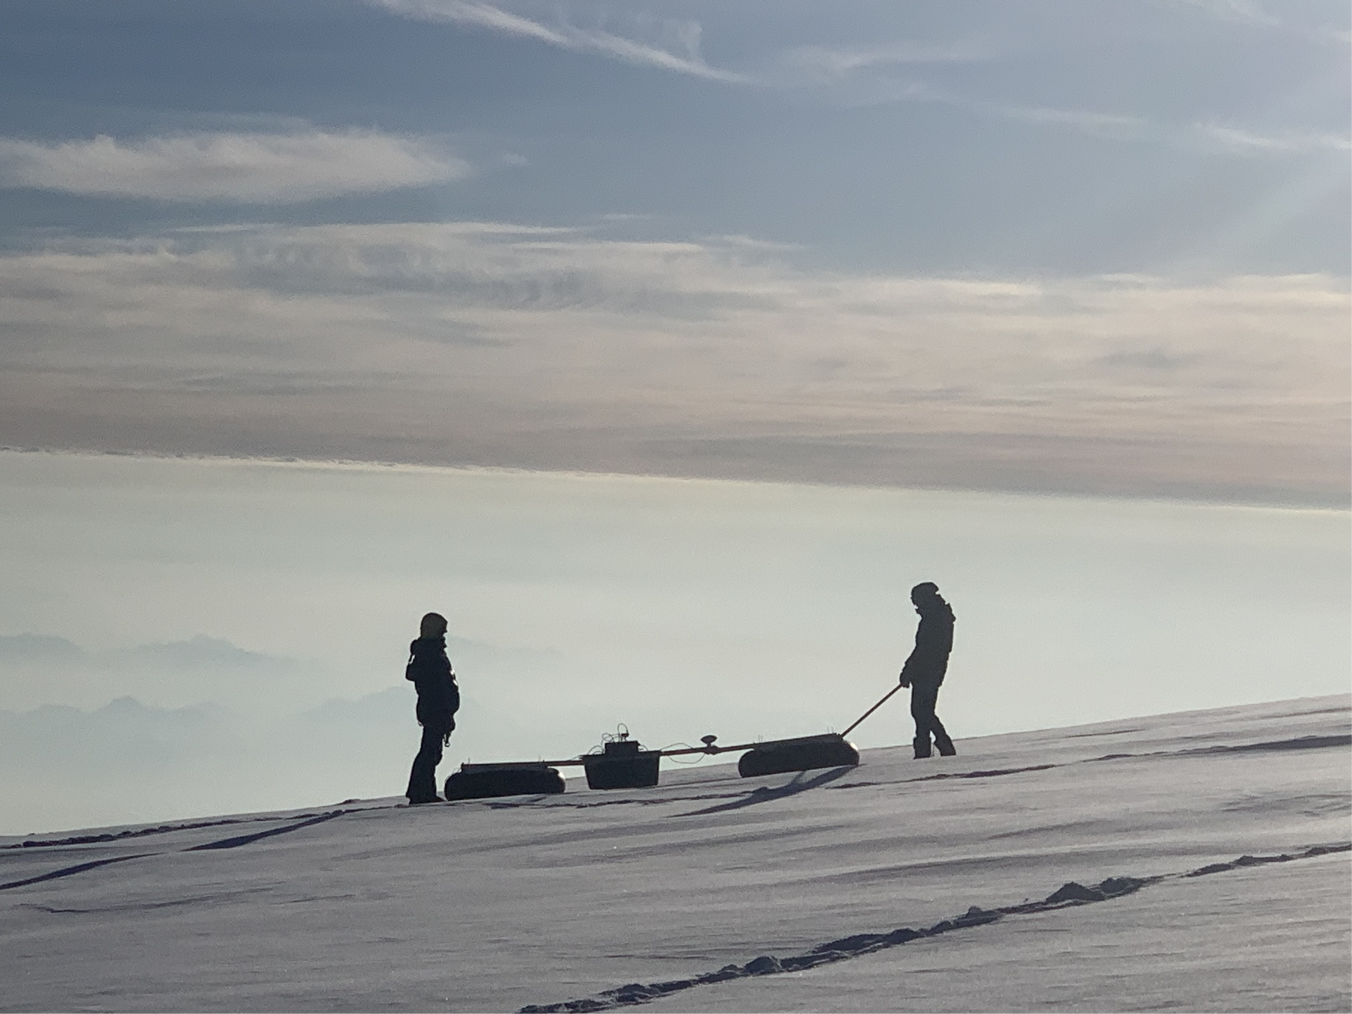
\includegraphics[width=0.99\textwidth]{Figures/General/FieldPhotos/GPRColle.png}
      \end{PointSix}
\end{frame}

\begin{frame}
    \begin{PointSix}{Who's teaching?}
        \alert{Introduction to Geophysics - R. Drews}
        \small Prof. for Geophysics since 2022
        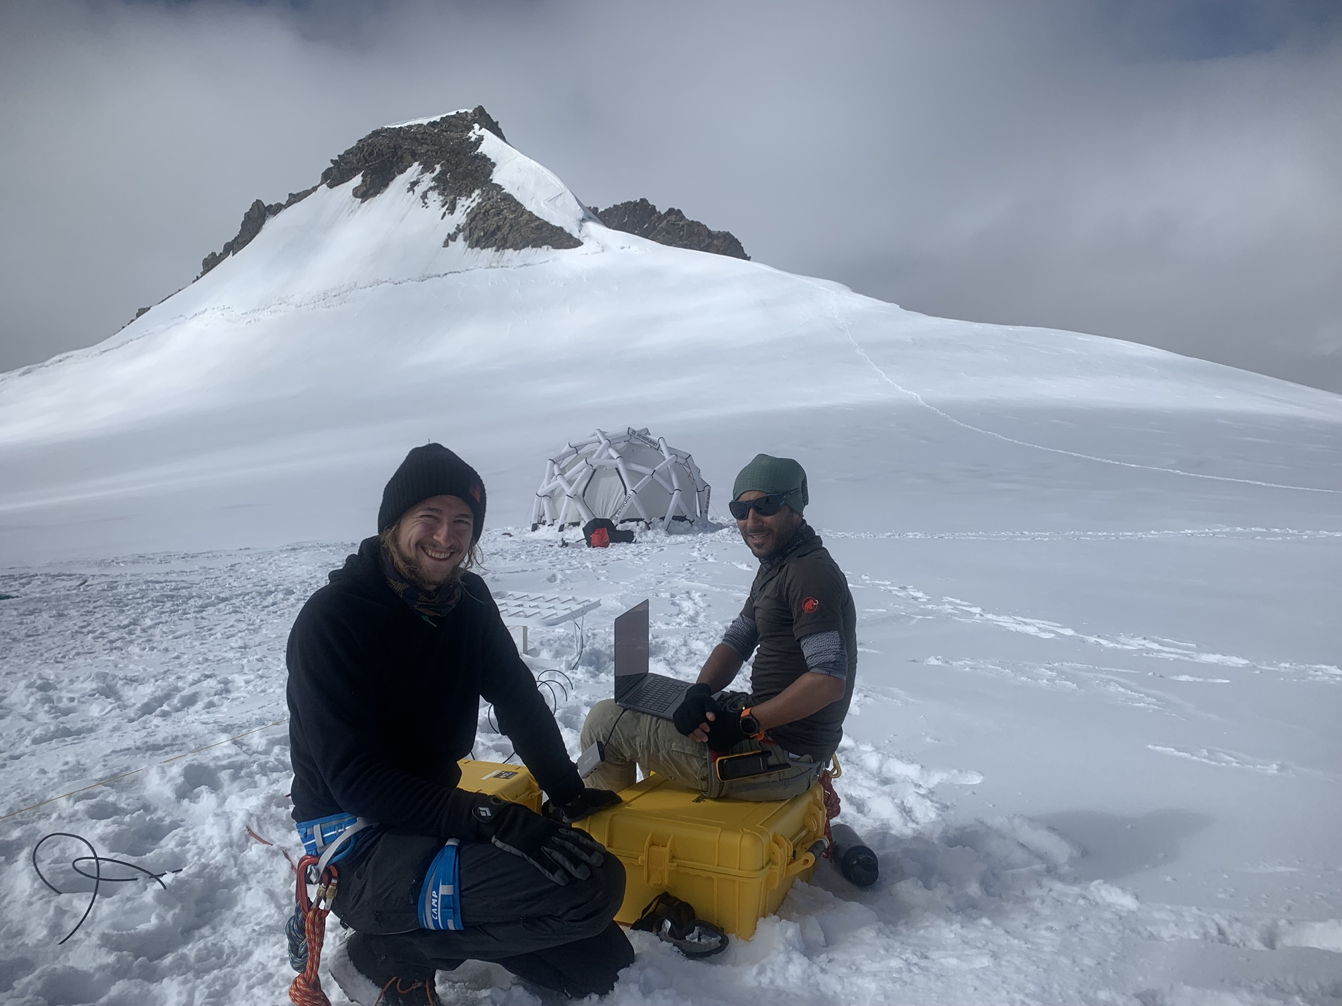
\includegraphics[width=0.99\textwidth]{Figures/General/FieldPhotos/GPRColle2.png}
      \end{PointSix}
\end{frame}

\begin{frame}
    \begin{PointSix}{Who's teaching?}
        \alert{Introduction to Geophysics - R. Drews}
        \small Prof. for Geophysics since 2022
        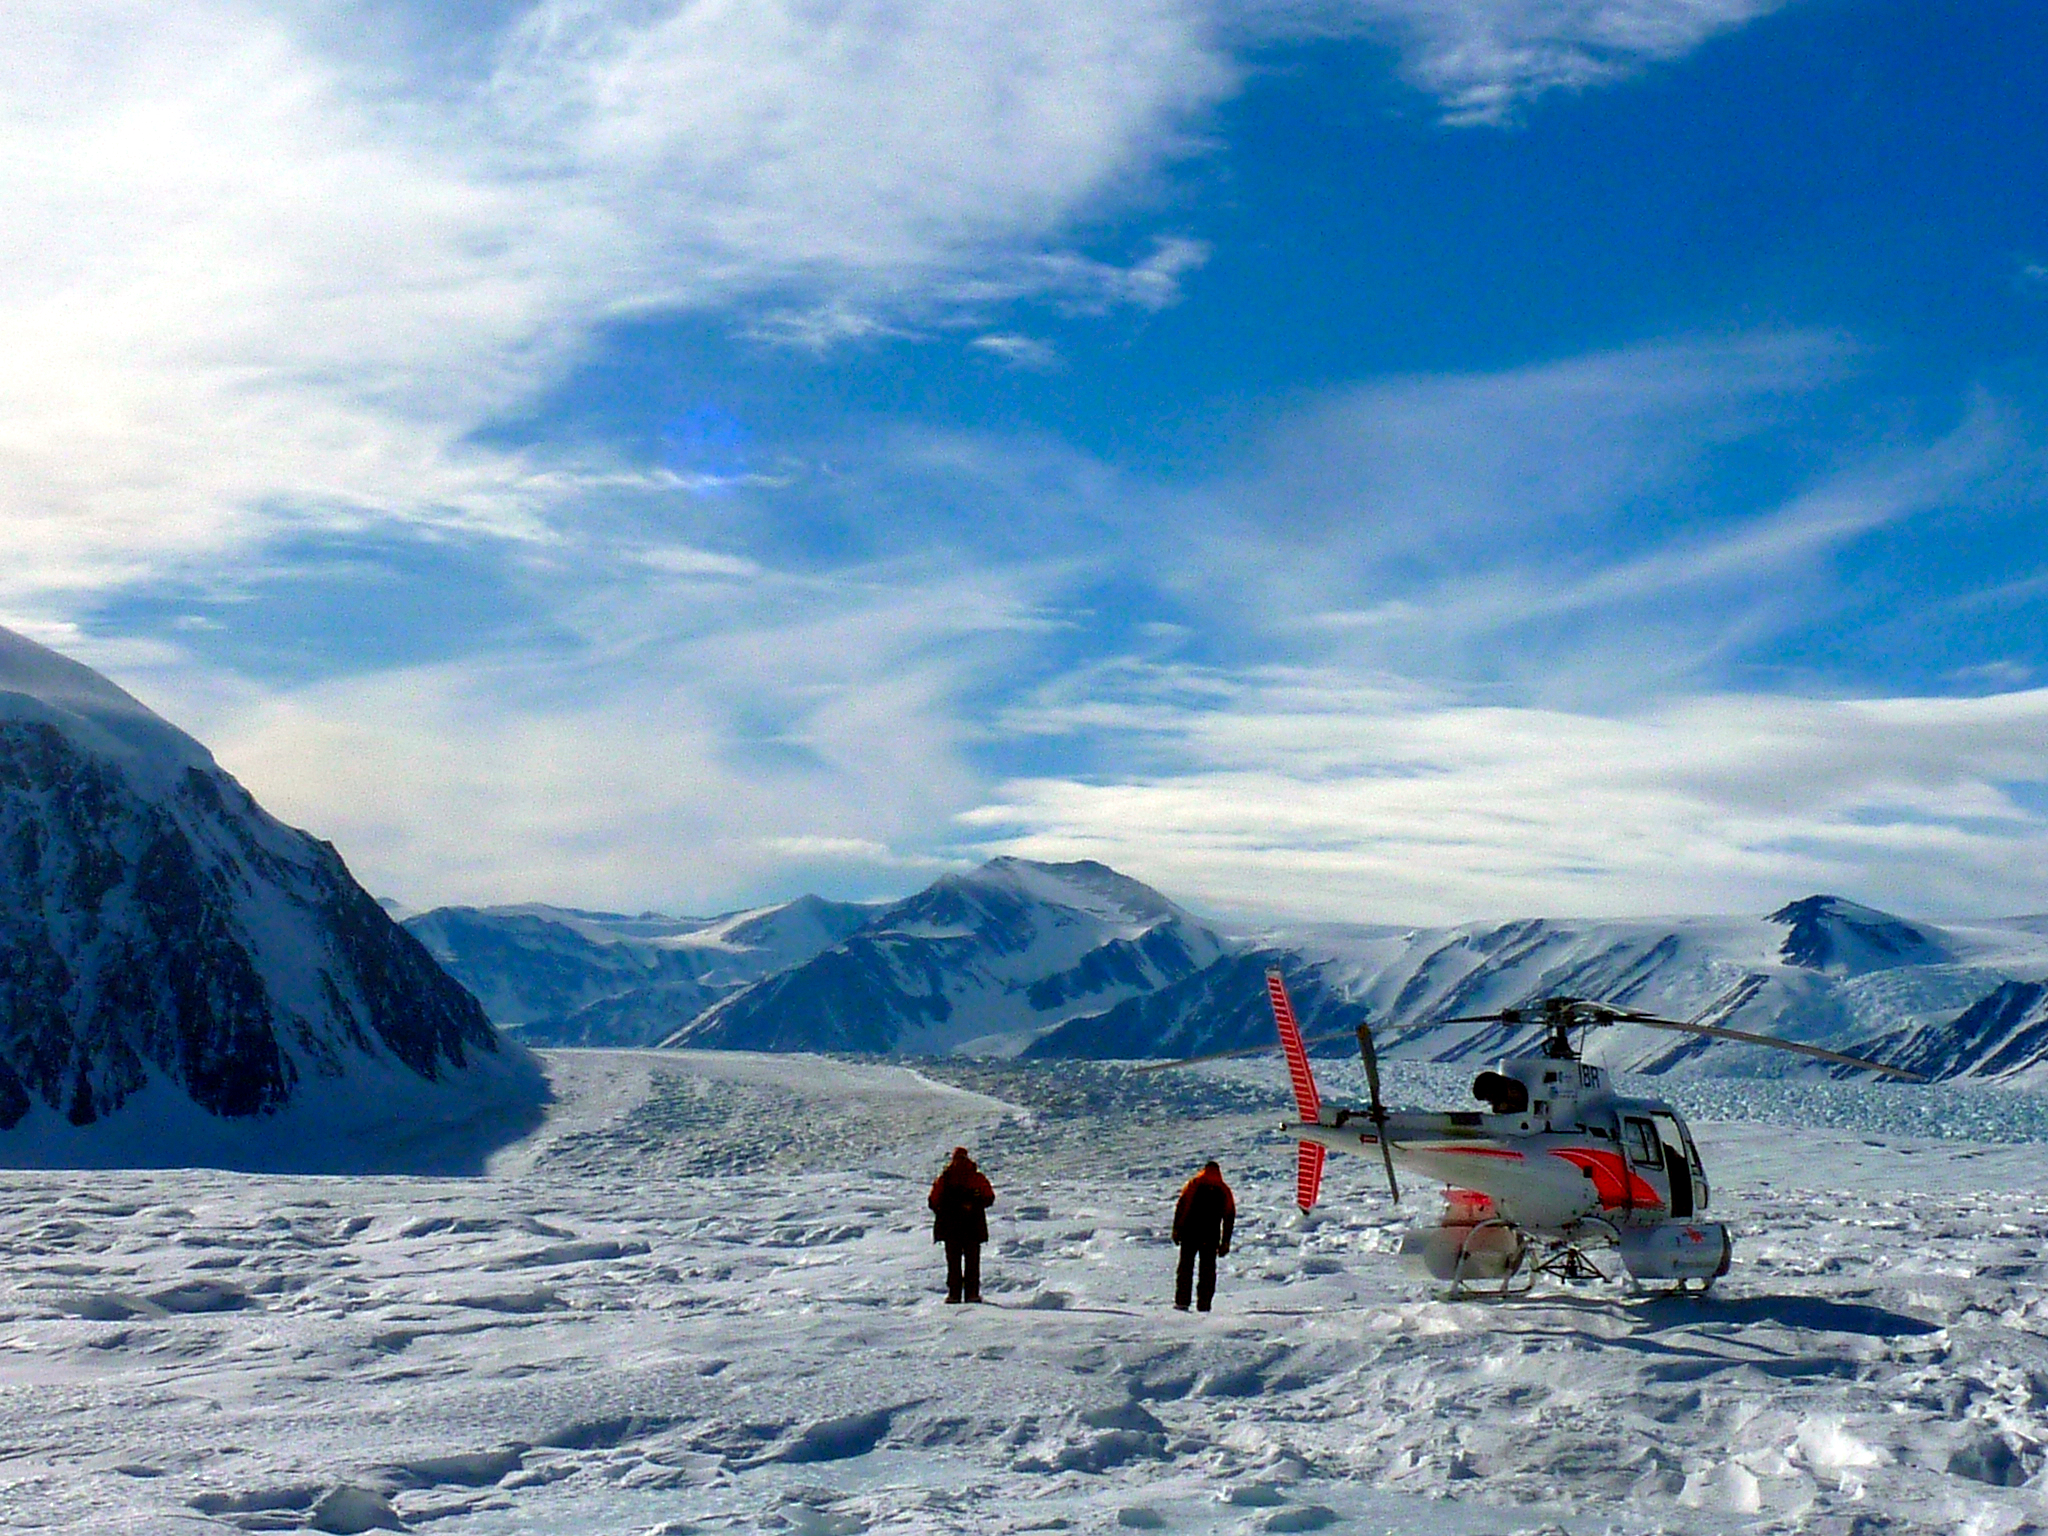
\includegraphics[width=0.99\textwidth]{Figures/General/FieldPhotos/PriestleyHelicopter.JPG}
      \end{PointSix}
\end{frame}

\begin{frame}
    \begin{PointSix}{Who's teaching?}
        \alert{Introduction to Geophysics - R. Drews}
        \small Prof. for Geophysics since 2022
        \includegraphics[width=0.99\textwidth]{Figures/General/FieldPhotos/GPRI.jpg}
      \end{PointSix}
\end{frame}

\begin{frame}
    \begin{PointSix}{Who's teaching?}
        \alert{Introduction to Geophysics - R. Drews}
        \small Prof. for Geophysics since 2022
        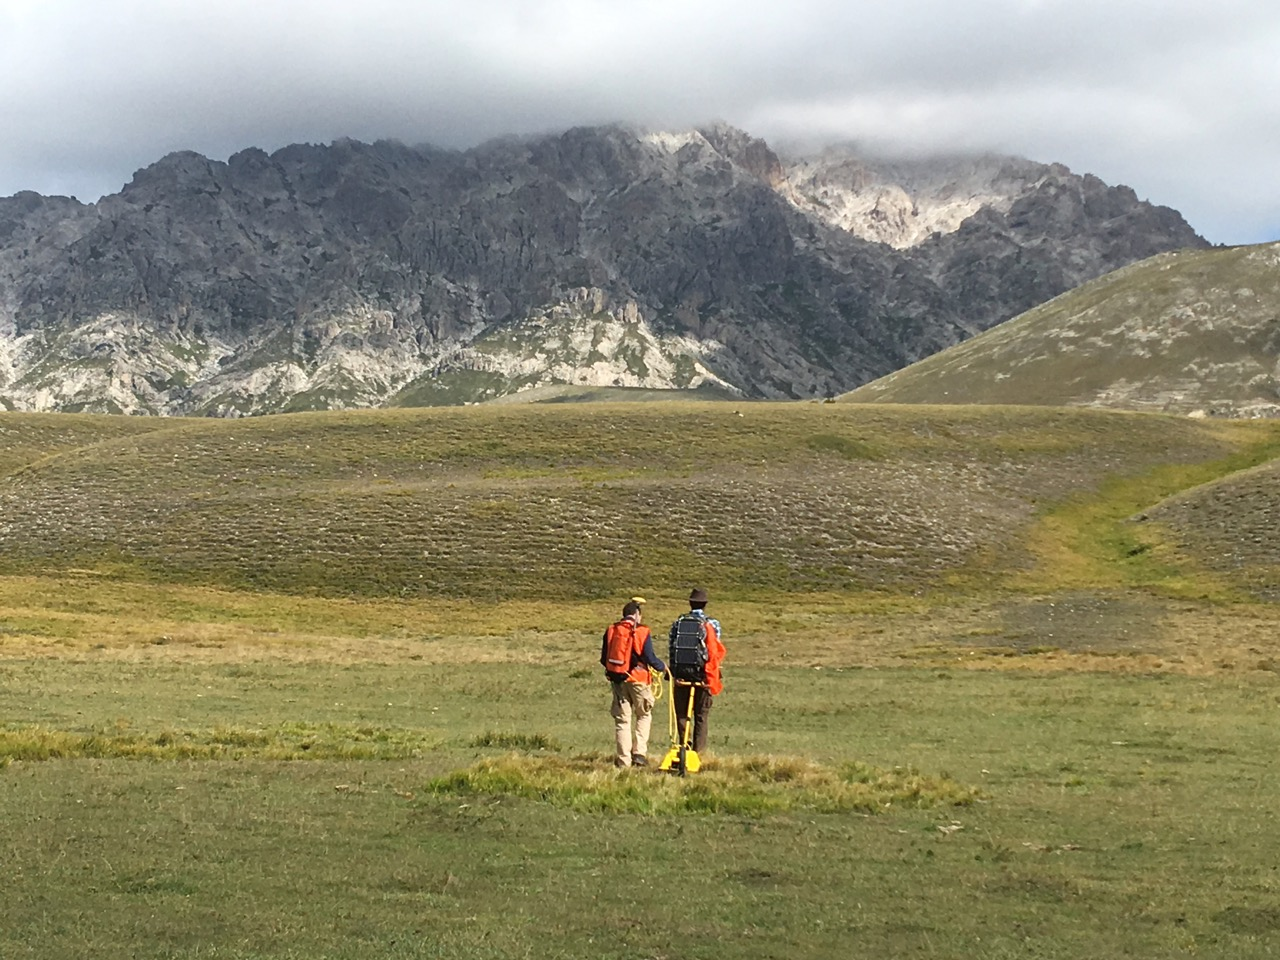
\includegraphics[width=0.99\textwidth]{Figures/General/FieldPhotos/ApenninsGPR.jpg}
      \end{PointSix}
\end{frame}


\begin{frame}
    \begin{PointSix}{What are we teaching?}
        \small
        \alert{Geophysics} is a branch of earth science dealing with the physical processes and phenomena occurring especially in the earth and in its vicinity.\\
        \vspace{0.25cm}
        \tiny [Merriam-Webster]\\
        \small
        \vspace{2.25cm}
        \alert{Applied Geophysics} is a branch of Geophysics dealing with different observational methods imaging the sub-surface.\\
        \vspace{0.25cm}
        \tiny [The lecture focus will be here.]
    \end{PointSix}
\end{frame}

\begin{frame}
    \begin{PointSix}{What are we teaching?}
        \small
        \alert{Applied Geophysics} contains, e.g, gravity, magnetics, electrics, electrical induction, electromagnetics (radar), seismics.\\
        \vspace{0.25cm}
        \tiny [Focus on physical principals rather than aquisition specifics.]
    \end{PointSix}
\end{frame}

\begin{frame}
    \begin{PointSix}{Example: Seismics}
        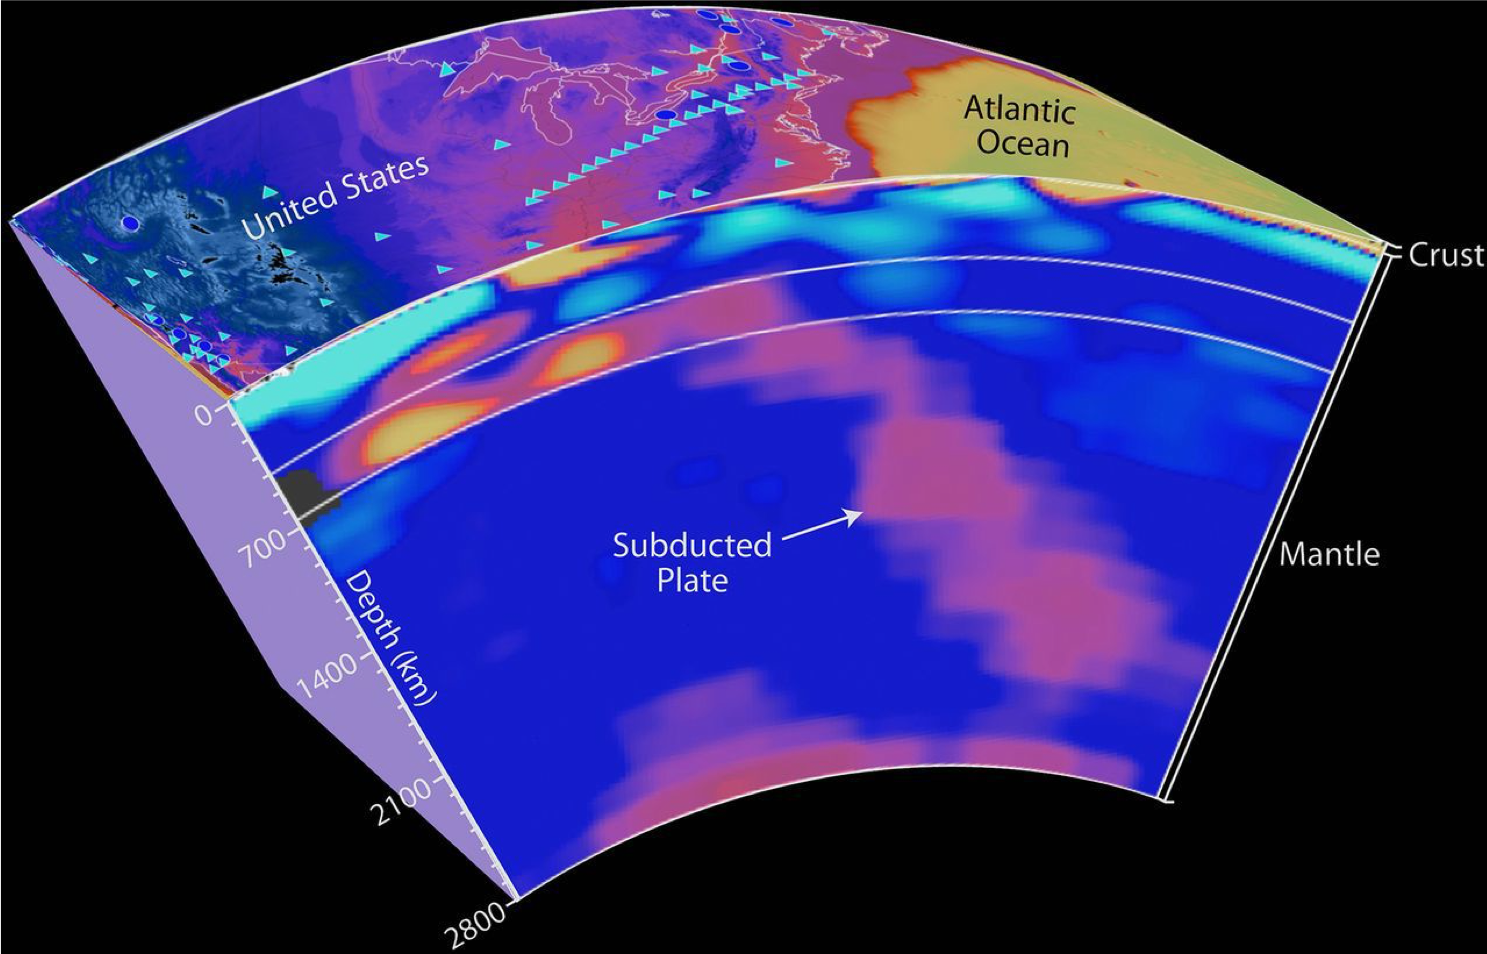
\includegraphics[width=0.99\textwidth]{Figures/General/GeophysExamples/Seismics_SvdLEE_Evanston_IL.png}
        \tiny[S. van der Lee, Northwestern University, Evanston, IL]
        %Data gathered by a network of seismic instruments (red) have enabled researchers to discern a region of relatively cold, stiff rock (shades of green and blue) beneath eastern North America. This is likely to be the remnants of an ancient tectonic plate. Image credit: Suzan van der Lee (Northwestern University, Evanston, IL).

    \end{PointSix}
\end{frame}

\begin{frame}
    \begin{PointSix}{Example: Magnetics}
        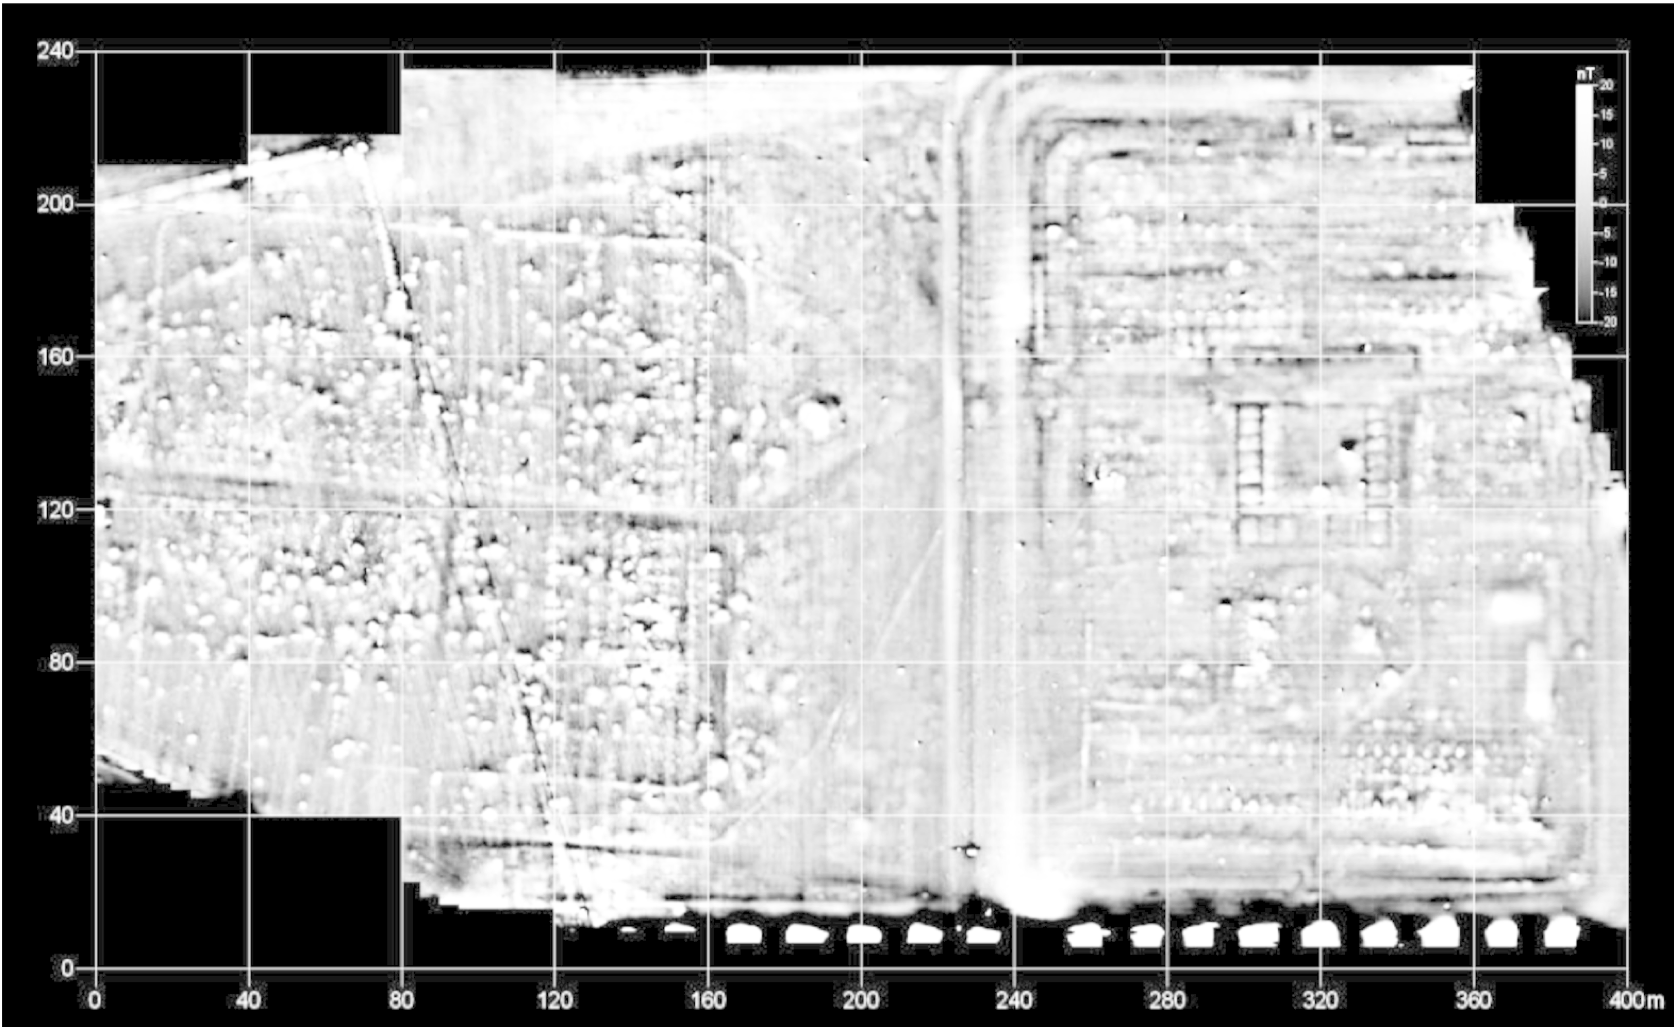
\includegraphics[width=0.99\textwidth]{Figures/General/GeophysExamples/Magnetics1_FassbinderBADS.png}
        \tiny[Fassbinder, Bavarian Academy of Sciences]
           \end{PointSix}
\end{frame}
\begin{frame}
    \begin{PointSix}{Example: Magnetics}
        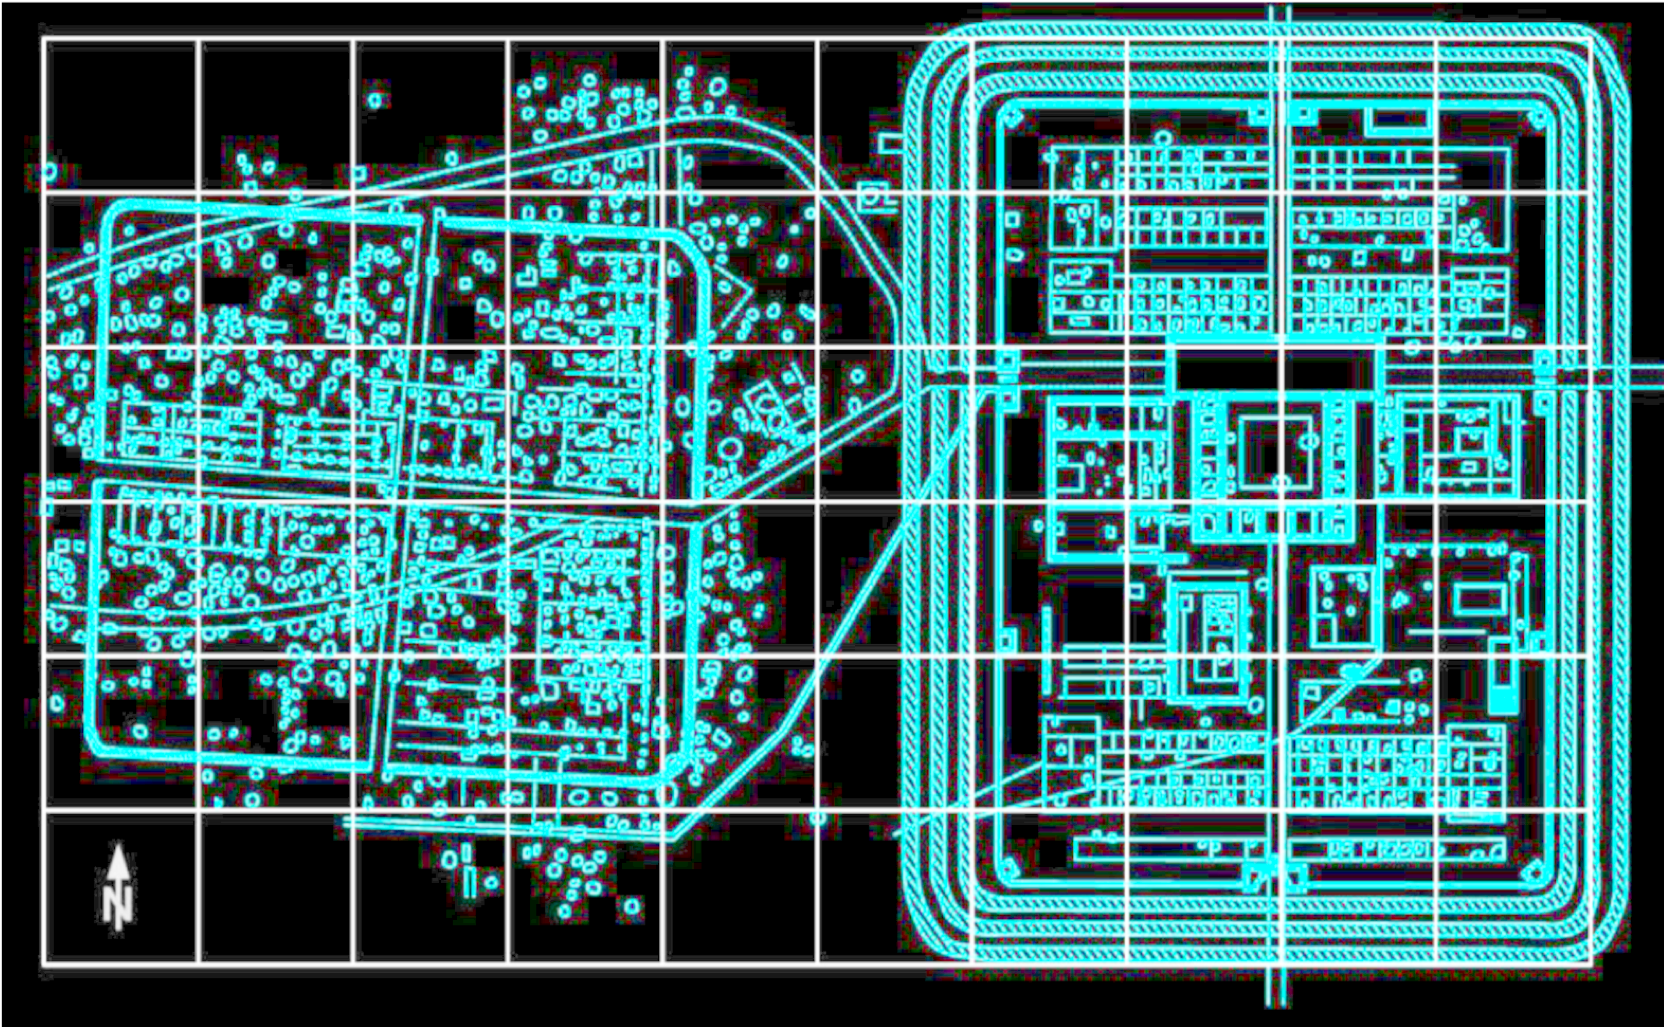
\includegraphics[width=0.99\textwidth]{Figures/General/GeophysExamples/Magnetics2_FassbinderBADS.png}
        \tiny[Fassbinder, Bavarian Academy of Sciences]
           \end{PointSix}
\end{frame}
\begin{frame}
    \begin{PointSix}{Example: Geoelectrics}
        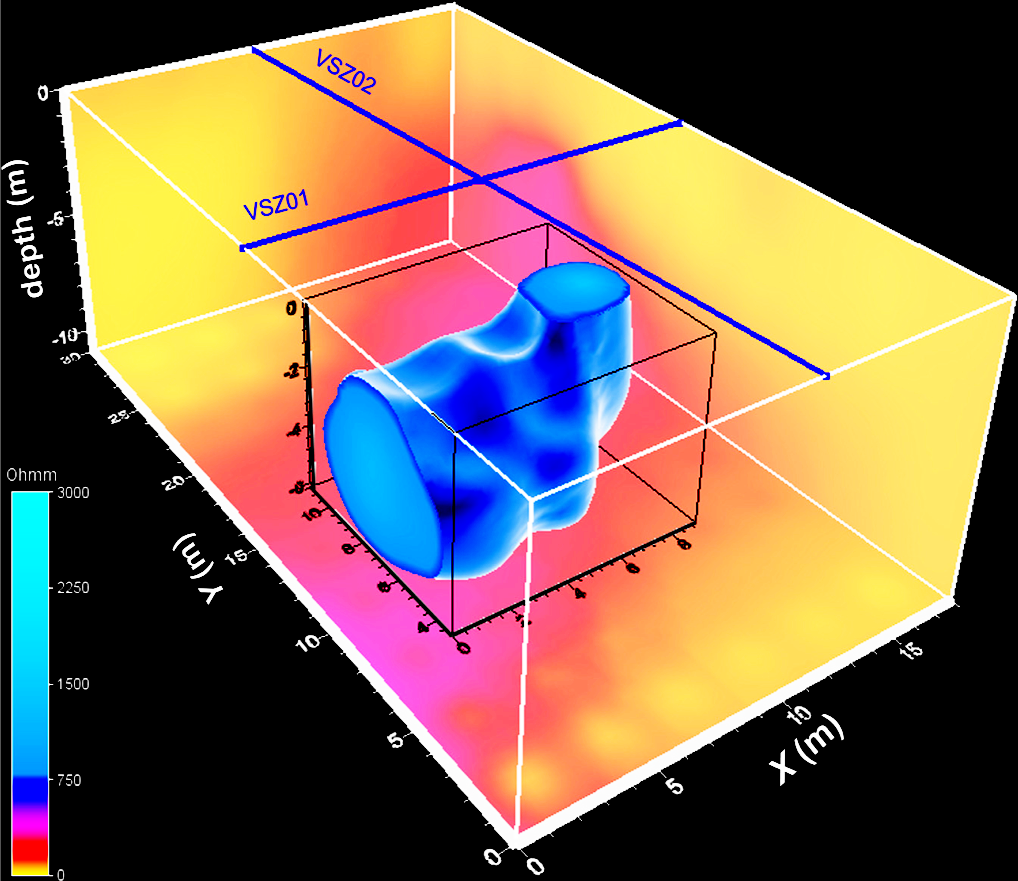
\includegraphics[width=0.9\textwidth]{Figures/General/GeophysExamples/DCElectricsSinkhole_Plank2019NearSurfaceGeophys_Reversed.png}

        \tiny[Plank et al., Near Surface Geophysics, 2019]
        %Volumetric interpretation of the former sinkhole at 900 Ωm isovalue. The resistivity scale is not artificially distorted. The yellow lines indicate the traces of 2D geoelectric survey lines. The crossing point is not above the sinkhole.
        \end{PointSix}
\end{frame}

\begin{frame}
    \begin{PointSix}{Example: Gravity}
        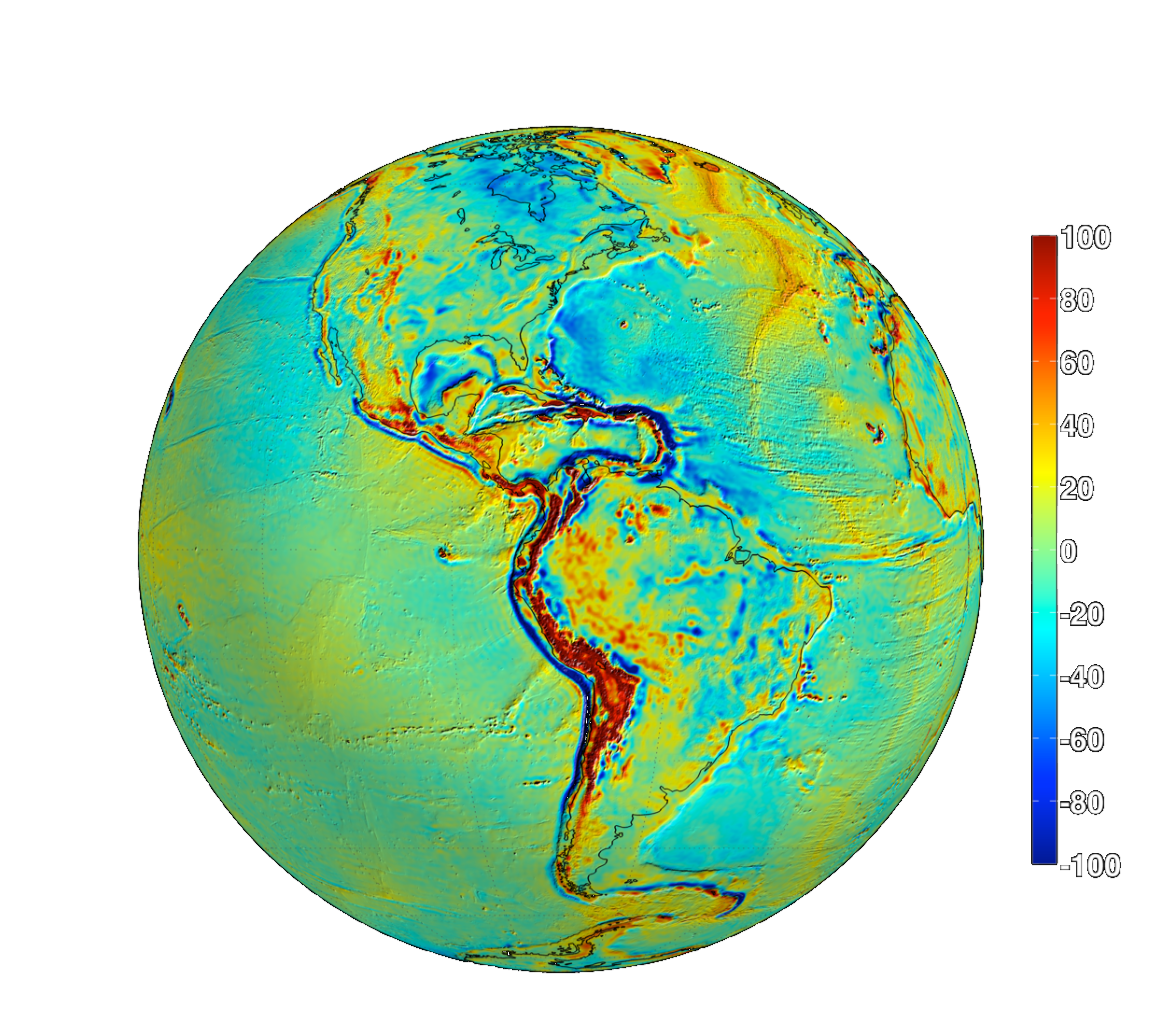
\includegraphics[width=0.90\textwidth]{Figures/Gravity/Exported/Grace_JPLCaltect_FODT10_WithoutPeople.png}
    \end{PointSix}
\end{frame}



\begin{frame}
    \small
    \begin{PointSix}{How do we teach? }
        \begin{itemize}
            \item Video Lectures or Plenum (Tuesdays)
            \item Exercises \& 1-1-Interaction (Thursdays)
            \item Applied Exercises (Magnetics, Electrics, Seismics)
        \end{itemize}
    \end{PointSix}
\end{frame}

\begin{frame}
    \begin{PointSix}{How do we teach?}
        \small
        \alert{Learning Goals}
        \begin{itemize}
            \item Obtain a broad overview of geophysical methods for sub-surface imaging.
            \item Understand the underlying physical principles.
            \item Learn how to think logically \& quantitatively.
        \end{itemize}
    \end{PointSix}
\end{frame}

\begin{frame}
    \begin{PointThree}{How do we teach?}
        \small
        \alert{Expectations}
        \begin{itemize}
            \item Be prepared.
            \item Ask questions.
            \item Do the work.
        \end{itemize}
    \end{PointThree}
\end{frame}

\begin{frame}
    \begin{PointSix}{How do we teach? $\rightarrow$ Ilias}
        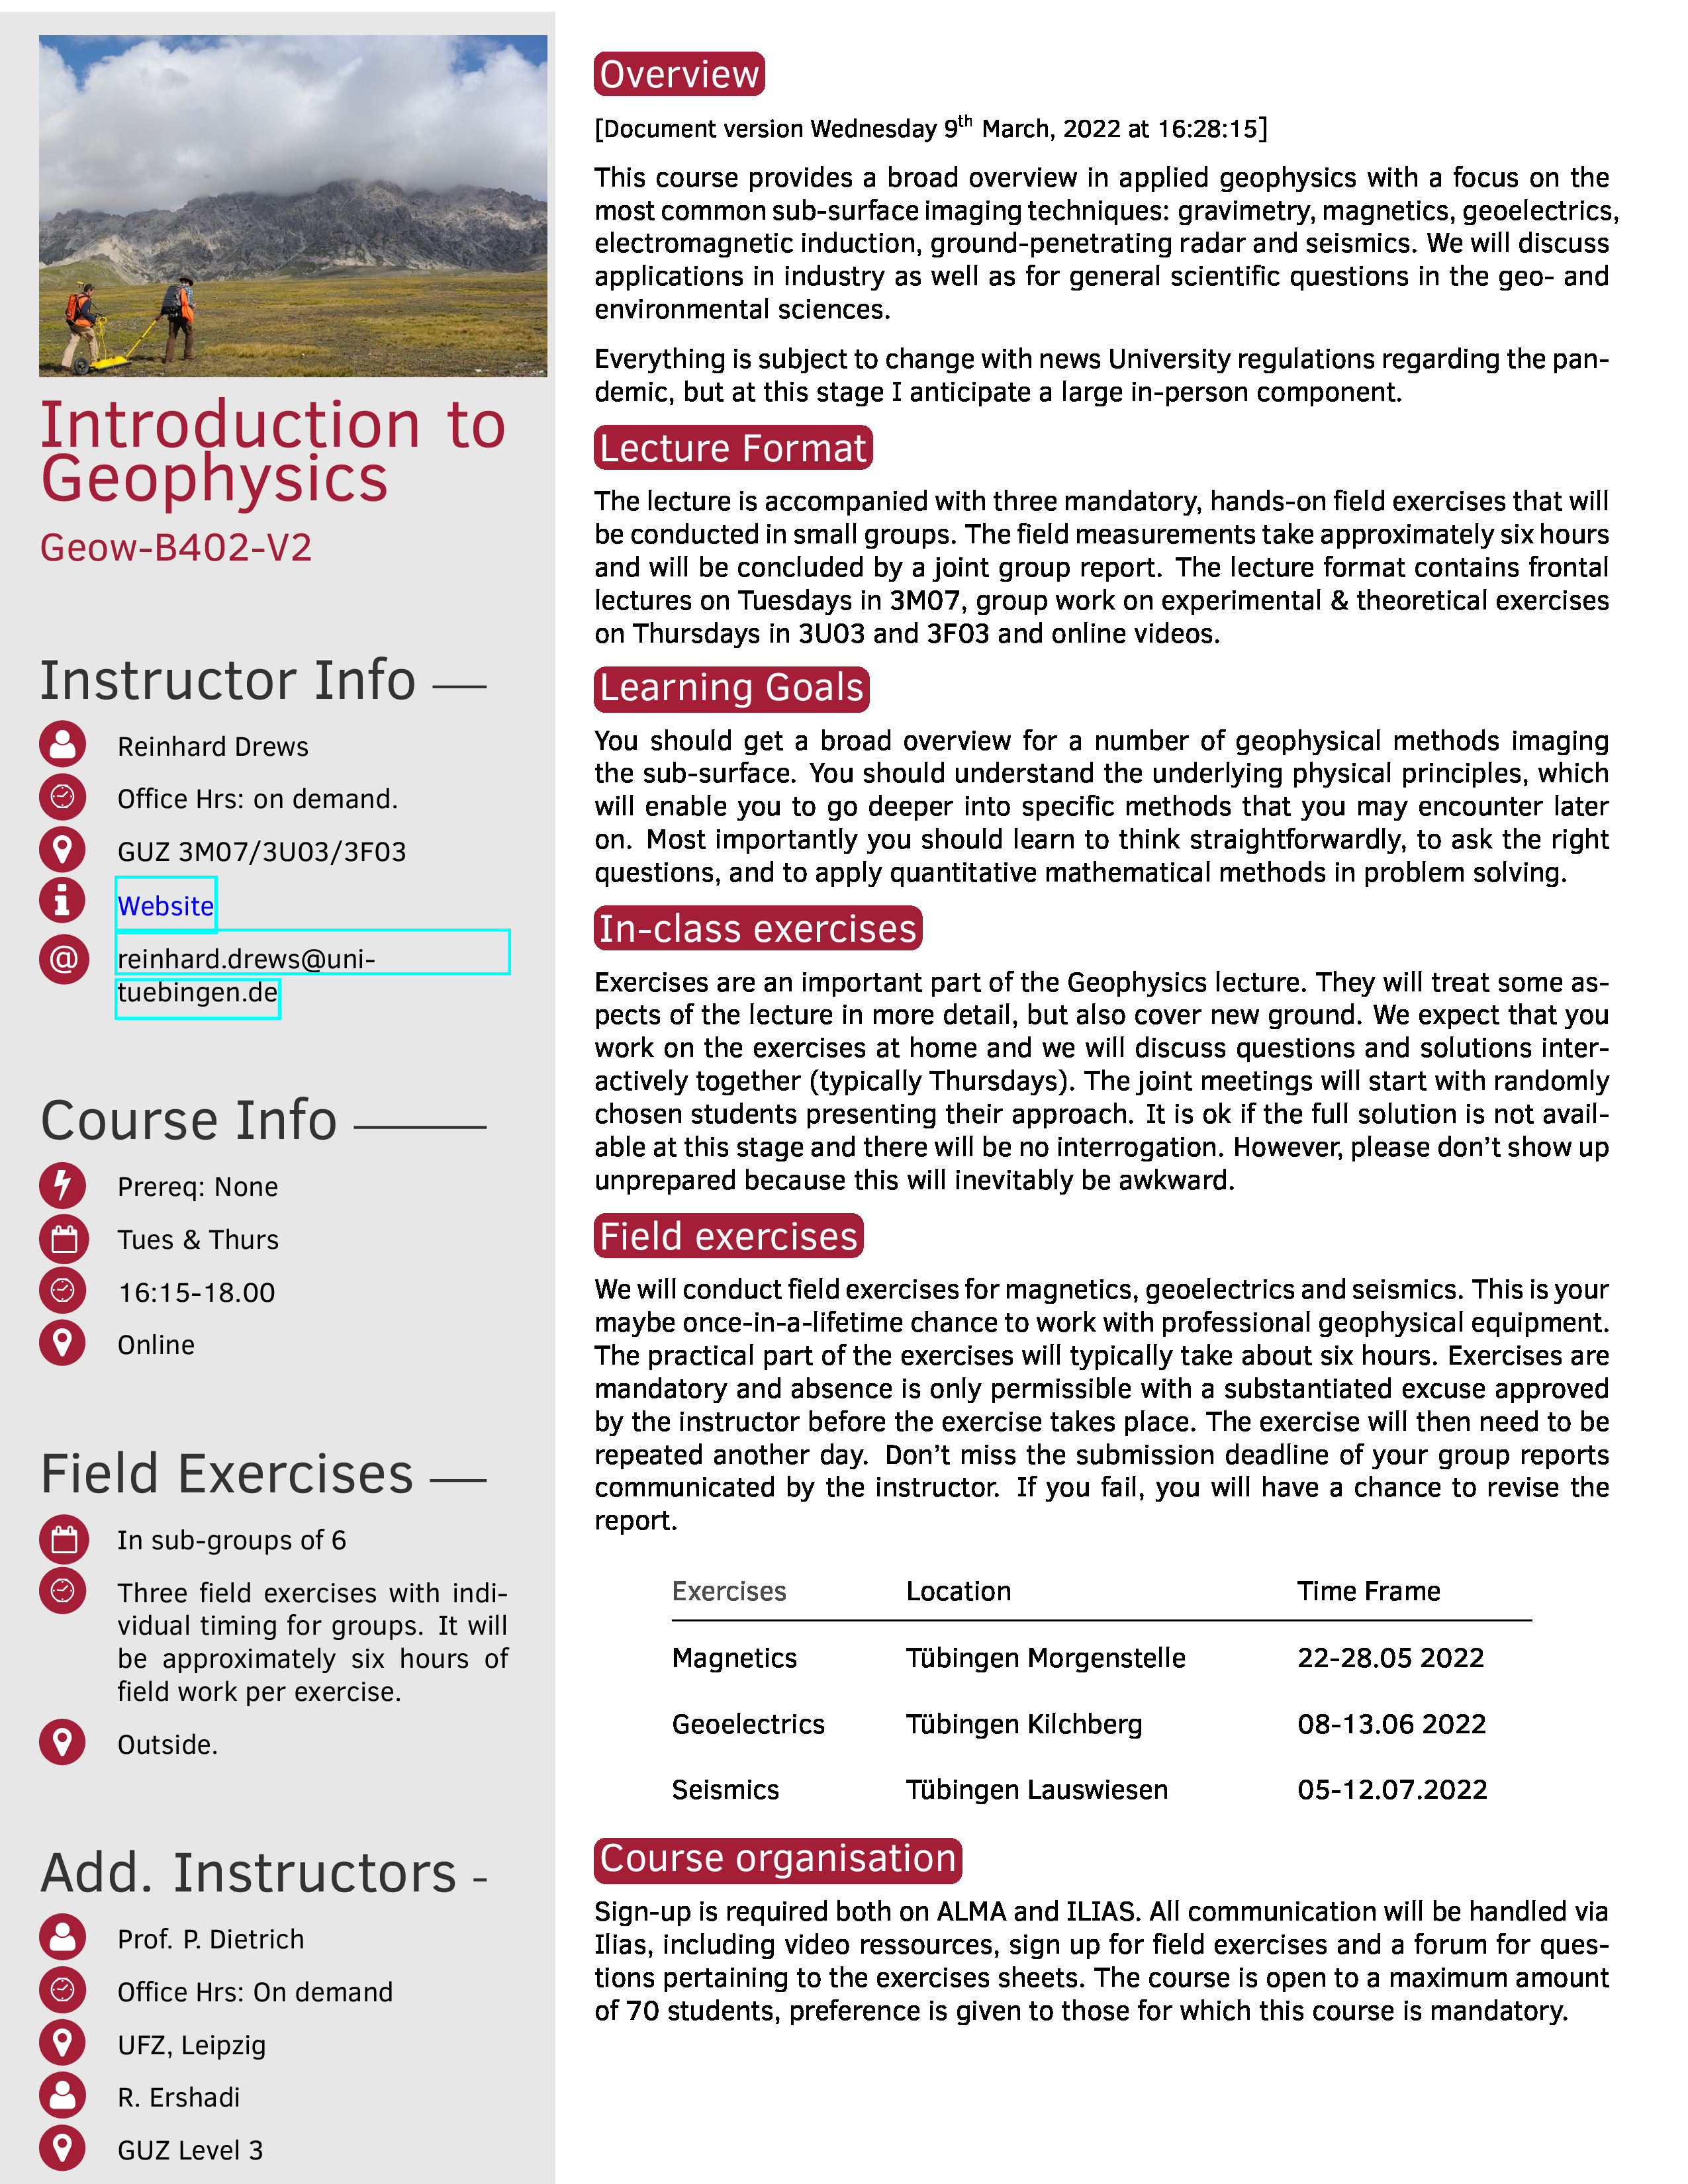
\includegraphics[width=0.90\textwidth]{Figures/General/LectureOutline_PageOne.jpg}
    \end{PointSix}
\end{frame}
\begin{frame}
  \begin{PointSix}{Learning Goals}
    \alert{Learning goals today:}
    \begin{itemize}
      \item The gravitational force, its potential field, and how to measure it.
      \item The reference gravitational field of the Earth.
    \end{itemize}
  \end{PointSix}
  \end{frame}

\begin{frame}
  \begin{PointSix}{Example: Global variability}
      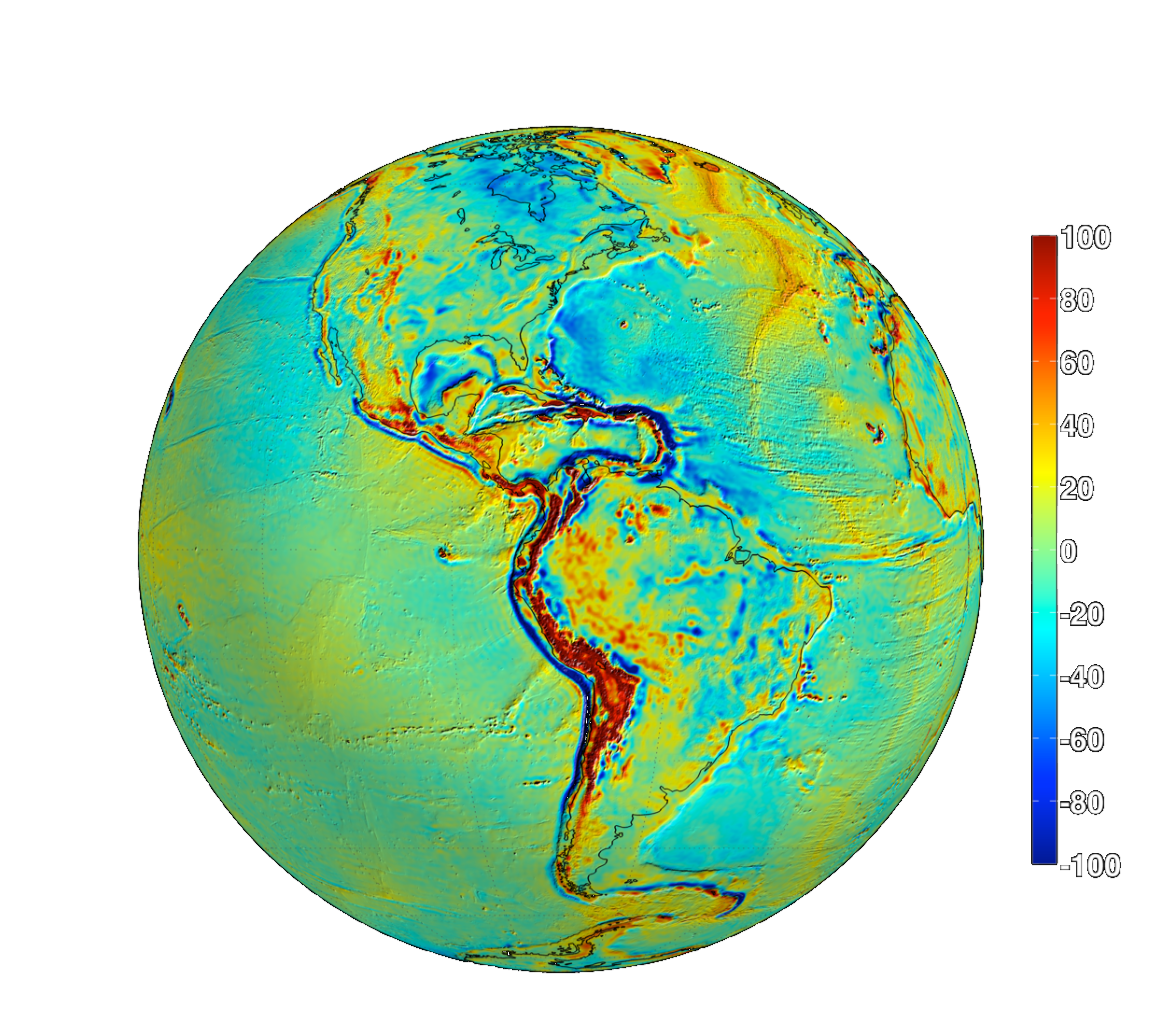
\includegraphics[width=0.99\textwidth]{Figures/Gravity/Exported/Grace_JPLCaltect_FODT10_WithoutPeople.png}
  \end{PointSix}
\end{frame}

\begin{frame}
  \begin{PointSix}{Example: Global variability}
  \centering
  \small Your mass is constant but your weight is not.
  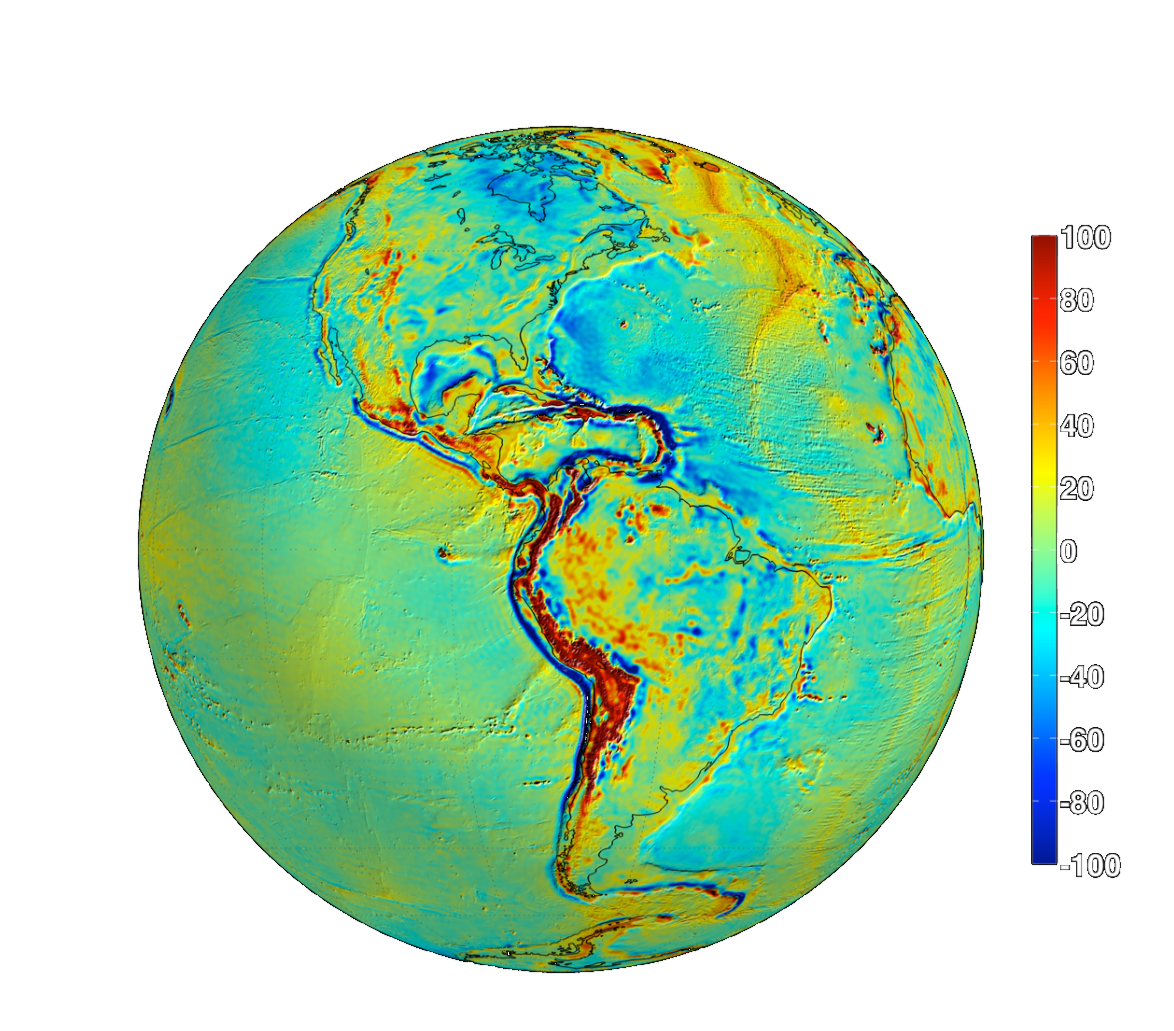
\includegraphics[width=0.99\textwidth]{Figures/Gravity/Exported/Grace_JPLCaltect_FODT10_WithPeople.png}
  \end{PointSix}
\end{frame}


\begin{frame}
\begin{ThreeCols}{What is a force?}{
  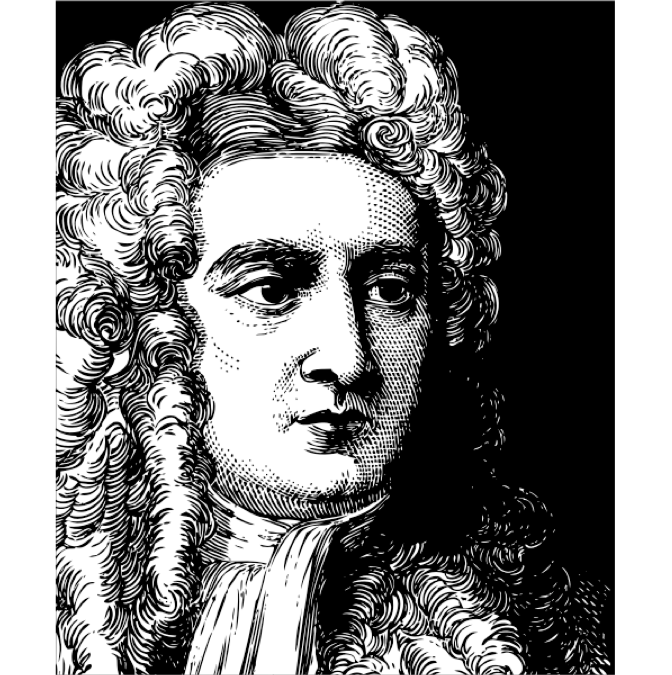
\includegraphics[width=0.8\textwidth]{Figures/Gravity/Exported/Newton_PD_GJohnson.png} \centering \tiny [Newton (1642-1726) / G. Johnson.]}
  \scalebox{1.5}{%
      $
      \vec{F} = m \vec{g}
      $
  }
  \scalebox{0.6}{\parbox{\linewidth}{
      \begin{align*}
      &\vec{F}:\,\text{Force}\,(\text{N};\,\text{kg}\,\text{m}\,\text{s}^{-2})\\
      &\vec{g}:\,\text{Acceleration}\,(\text{m}\,\text{s}^{-2})\\
      &\text{m}:\,\text{Mass (kg)}
      \end{align*}
  }}
\end{ThreeCols}
\end{frame}

\begin{frame}
  \begin{ThreeCols}{The gravitational force}{
      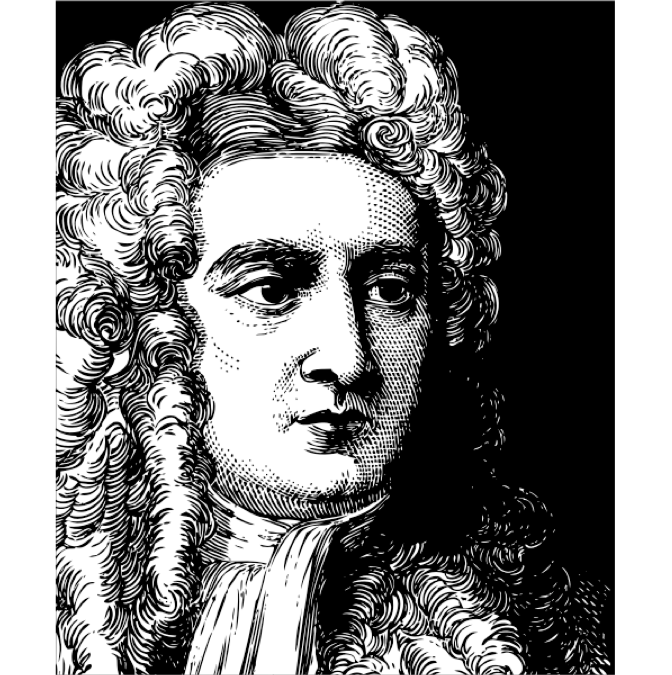
\includegraphics[width=0.8\textwidth]{Figures/Gravity/Exported/Newton_PD_GJohnson.png} \centering \tiny [Newton (1642-1726) / G. Johnson.]}
      \scalebox{1.5}{%
          $
          \vec{F} = G\frac{mM}{r^2}\hat{r}
          $
      }
      \scalebox{0.6}{\parbox{\linewidth}{
          \begin{align*}
          &G=6.674 \cdot 10^{-11}\,\text{(}\,m^3 kg^{-1} s^{-2}\text{)}\\
          &\hat{r}:\,\text{unit vector}\\
          &r:\,\text{distance between point masses}
          \end{align*}
      }}
      \begin{tikzpicture}
          \coordinate (A) at (1,2);
          \coordinate (B) at (2,4);

          \draw [fill=white] (A) circle (8pt) node [left,xshift=-0.5cm] {M};
          \draw [fill=white] (B) circle (4pt) node [left,xshift=-0.5cm] {m};


          \draw[-latex,thick,Karminrot,->] (A) -- (B) node[midway,left,rotate=0] {$r$};
          \draw [-latex,thick, Karminrot] (B) -- (A);
          \end{tikzpicture}
  \end{ThreeCols}
  \end{frame}

  \begin{frame}
      \begin{PointSix}{Example: The gravitational constant}
          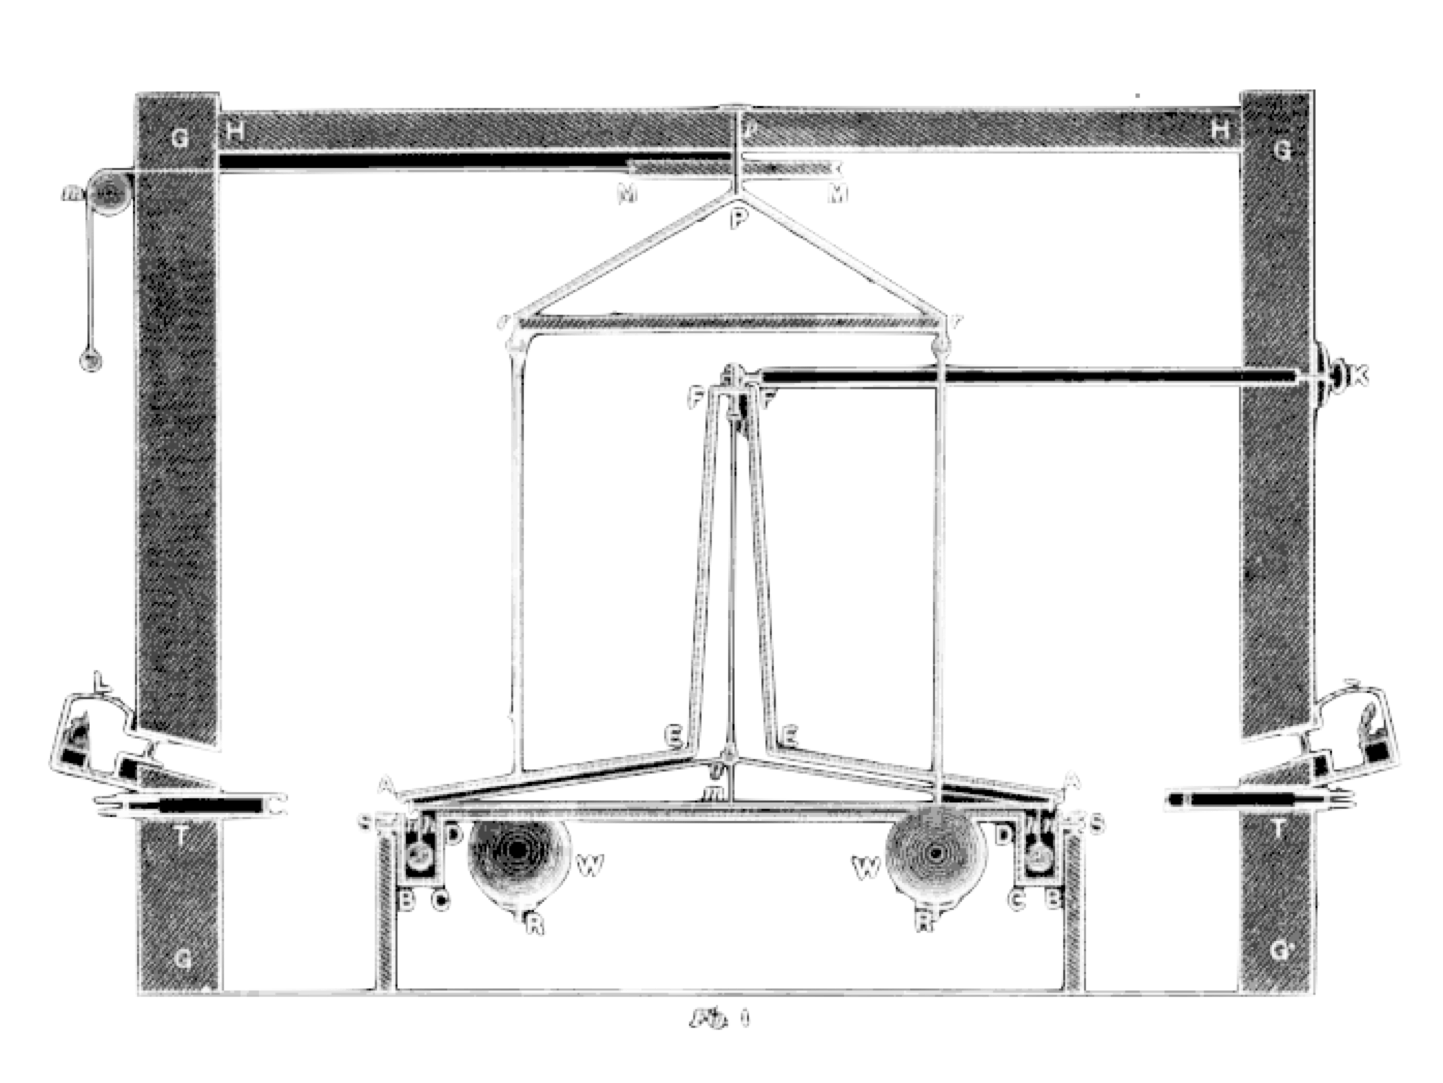
\includegraphics[width=0.99\textwidth]{Figures/Gravity/Exported/Cavendish_PNAS1798.png}
          \centering
          \tiny Cavnedish, PNAS, 1798
      \end{PointSix}
  \end{frame}
  \begin{frame}
      \begin{PointSix}{Example: The gravitational constant}
          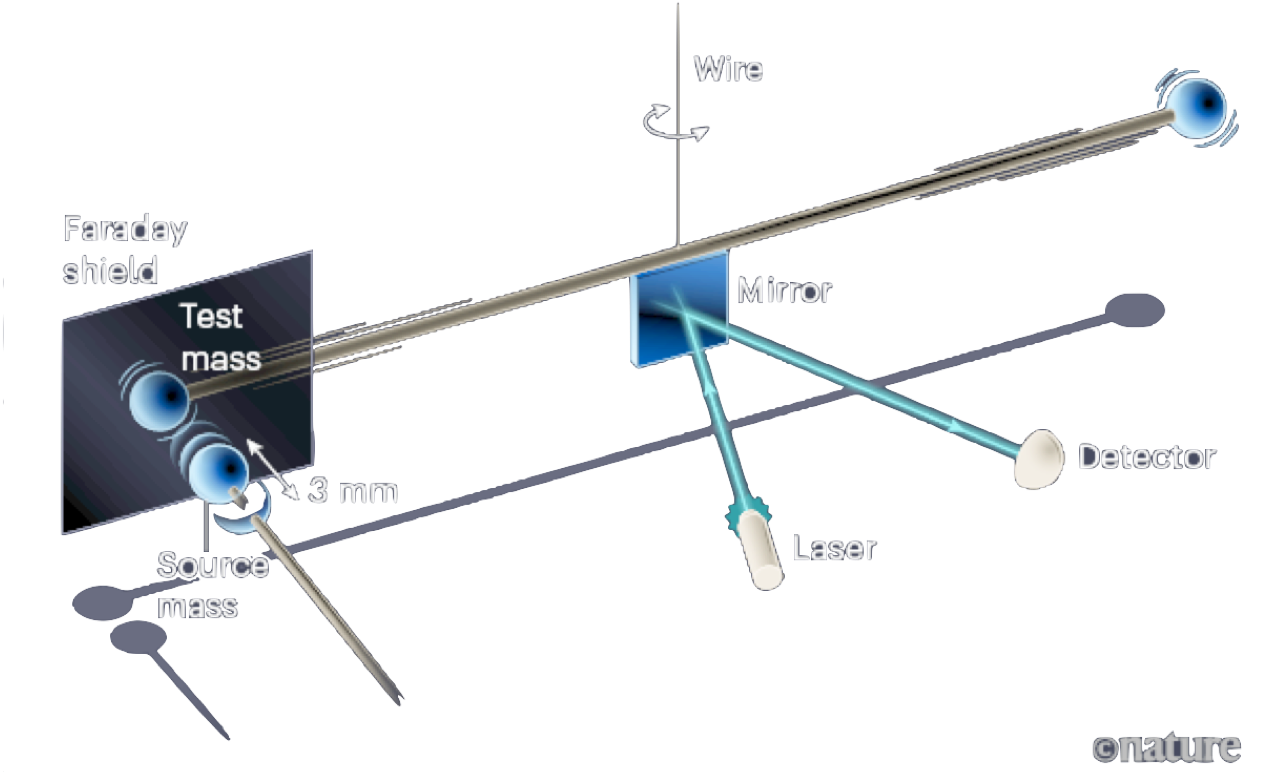
\includegraphics[width=0.99\textwidth]{Figures/Gravity/Exported/MeasuringG_Westphal_Nature2021.png}
          \centering
          \tiny Westphal et al., Nature, 2021\\
          \normalsize G is the worst known constant in physics. Why?
      \end{PointSix}
  \end{frame}

\begin{frame}
\begin{PointSix}{Example: Measuring acceleration}
  \begin{minipage}[t]{0.3\textwidth}
    
\includegraphics[width=\textwidth]{Figures/General/ScarySmiley_Kindpng.png}
    \end{minipage}\begin{minipage}[]{0.7\textwidth}
  \centering
  \begin{align*}
  &\vec{F} = m \vec{g} \\
  &\vec{F} = G\frac{mM}{r^2}\hat{r} \\
  &\rightarrow \vec{g} = G\frac{M}{r^2}\hat{r} \\
  &\rightarrow \frac{d^2\vec{x}}{dt^2} = G\frac{M}{r^2}\hat{r} \\
  \end{align*}
\end{minipage}
  \centering
  This is a differential equation.

\end{PointSix}
\end{frame}

\begin{frame}
\begin{PointSix}{Example: Measuring acceleration}
  \begin{minipage}[t]{0.3\textwidth}
    
\includegraphics[width=\textwidth]{Figures/General/IcandothisSmiley_Kindpng.png}
    \end{minipage}\begin{minipage}[]{0.7\textwidth}
  \centering
  \begin{align*}
  &\frac{d^2\vec{x}}{dt^2} = G\frac{M}{R_E^2} \approx const. \\
  \end{align*}
\end{minipage}
 % \centering
  At the Earth's surface ($R_E$) g is close to constant and only vertical. (Later we will see that none of this is not quite true).

\end{PointSix}
\end{frame}

\begin{frame}
  \begin{PointSix}{Example: Measuring acceleration}
  \begin{tikzpicture}
      \begin{axis}[
        rdstyle,
        xlabel=time (s),
        ylabel={$g (m s^{-2})$},
        xmin=0,
        xmax=10,
        xtick={0,2,...,10},
        color=white,
        width=9cm,
      ]
        \addplot[domain=0:10,samples=10,color=Karminrot,line width=0.5mm] {x*0 +9.81};
        \node[] at (axis cs: 5,11) {$g = \frac{d^2}{dt^2}x(t)=\frac{GM}{R_e^2}\approx const.$};
      \end{axis}
    \end{tikzpicture}
  \end{PointSix}
\end{frame}

\begin{frame}
  \begin{PointSix}{Example: Measuring acceleration}
  \begin{tikzpicture}
      \begin{axis}[
        rdstyle,
        xlabel=time (s),
        ylabel={$v (m s^{-1})$},
        xmin=0,
        xmax=10,
        xtick={0,2,...,10},
        ytick=9.81,
        yticklabels={$c_1$},
        color=white,
        width=9cm,
      ]
        \addplot[domain=0:10,samples=10,color=Karminrot,line width=0.5mm] {x + 9.81};
        \node[] at (axis cs: 5,20) {$v = \int g dt=\frac{d}{dt}x(t)=\frac{GM}{R_e^2}t+c_1$};
      \end{axis}
    \end{tikzpicture}
  \end{PointSix}
\end{frame}

\begin{frame}
  \begin{PointSix}{Example: Measuring acceleration}
  \begin{tikzpicture}
      \begin{axis}[
        rdstyle,
        xlabel=time (s),
        ylabel={$x (m)$},
        xmin=0,
        xmax=10,
        xtick={0,2,...,10},
        ytick=9.81,
        yticklabels={$c_2$},
        color=white,
        width=9cm,
      ]
        \addplot[domain=0:10,samples=10,color=Karminrot,line width=0.5mm] {x^2 + 10};
        \node[] at (axis cs: 5,100) {$x(t) = \int v(t) dt=\frac{GM}{2R_e^2}t^2+c_1t+c_2$};
      \end{axis}
    \end{tikzpicture}
  \end{PointSix}
\end{frame}
\begin{frame}

\begin{PointSix}{Example: Measuring acceleration}
     \begin{align*}
       & x(t) = \frac{GM}{2R_e^2}t^2+c_1t+c_2 \\
     \end{align*}
     \begin{itemize}
      \item Setting, e.g., $c1=0$ (initial velocity) and $c_2=0$ (initial position) is quite convenient.
      \item This is the principal of a free-fall gravimeter.
    \end{itemize}
\end{PointSix}

\end{frame}

\begin{frame}
\begin{PointSix}{Exercises: Group-Work Thursdays}
  \begin{itemize}
    \item Thanks to the Greeks we know the radius $R_E$ for the Earth. However, its mass was unknown for a while.
    \item Go ahead and determine the mass of the Earth M with your Smartphone!
    \item \alert{There is an important first-order finding in Earth Sciences that you can (re-) discover. Which one?}
  \end{itemize}

\end{PointSix}
\end{frame}

\begin{frame}
\begin{PointSix}{Beyond point masses}
  \begin{tikzpicture}
    \coordinate (A) at (8,0);
    \coordinate (B) at (4,-3.5);
    \coordinate (C) at (5,-3.5);
    \coordinate (D) at (6,-3.5);
    \draw [thick] (0,0.0) -- (8,0.0);
    % drawing the node with shape=rectangle and anchor=center
    \node [draw, Karminrot, thick, shape=rectangle, minimum width=0.25cm, minimum height=0.25cm, anchor=center] at (B) {};
    \draw [->, thick] (0,0.0) -- (B) node[xshift=0.3cm,yshift=0.3cm,midway,left,rotate=-30] {$\vec{r}$};;

    \node[yshift=0.3cm] at (A) {\small Surface};

  \end{tikzpicture}
  $$
    \vec{F} = G\frac{dM}{r^2}\hat{r}
  $$
\small For a small mass dM the point mass approximation holds.
\end{PointSix}

\end{frame}



\begin{frame}
\begin{PointSix}{Beyond point masses}
  \begin{tikzpicture}
    \coordinate (A) at (8,0);
    \coordinate (B) at (4,-3.5);
    \coordinate (C) at (5,-3.5);
    \coordinate (D) at (6,-3.5);
    \draw [thick] (0,0.0) -- (8,0.0);
    % drawing the node with shape=rectangle and anchor=center
    \node [draw, Karminrot, thick, shape=rectangle, minimum width=0.25cm, minimum height=0.25cm, anchor=center] at (B) {};
    \foreach \i in {0,2,...,8}
    {
      \draw [->, thick] (0+\i,0.0) -- (B);
    }
    \node[yshift=0.3cm] at (A) {\small Surface};

  \end{tikzpicture}
  $$
    \vec{F} = G\frac{dM}{r^2}\hat{r}
  $$
  \small Profiling across a sub-surface target results in a gravity anomaly ($\rightarrow$ Exercises).
\end{PointSix}
\end{frame}

\begin{frame}
\begin{PointSix}{Beyond point masses}
  \begin{tikzpicture}
    \coordinate (A) at (8,0);
    \coordinate (B) at (4,-3.5);
    \coordinate (C) at (5,-3.5);
    \coordinate (D) at (6,-3.5);
    \draw [thick] (0,0.0) -- (8,0.0);
    \node[yshift=0.3cm] at (A) {\small Surface};

    \foreach \i in {-2,-1.5,...,2}
    {
      \foreach \j in {0,0.5}
      {
        \node [draw, Karminrot, thick, shape=rectangle, minimum width=0.25cm, minimum height=0.25cm, anchor=center] at (4-\i,-3.5-\j) {};
        \draw [->, thick] (0,0.0) -- (4-\i,-3.5-\j) ;

      }
    }

  \end{tikzpicture}
  $$
  \vec{F}(\vec{r}) = \sum_i G\frac{dM_i}{r_i^2}\hat{r_i}
  $$
  \small For $i$ point masses the effect adds up.
\end{PointSix}
\end{frame}

\begin{frame}
\begin{PointSix}{Beyond point masses}
  \begin{tikzpicture}
    \coordinate (A) at (8,0);
    \coordinate (B) at (4,-3.5);
    \coordinate (C) at (5,-3.5);
    \coordinate (D) at (6,-3.5);
    \draw [thick] (0,0.0) -- (8,0.0);
    \node[yshift=0.3cm] at (A) {\small Surface};

    \foreach \i in {-2,-1.5,...,2}
    {
      \foreach \j in {0,0.5}
      {
        \node [draw, Karminrot, thick, shape=rectangle, minimum width=0.25cm, minimum height=0.25cm, anchor=center] at (4-\i,-3.5-\j) {};
        \draw [->, thick] (2,0.0) -- (4-\i,-3.5-\j) ;

      }
    }
  \end{tikzpicture}
  $$
    \vec{F}(\vec{r}) = \sum G\frac{dM_i}{r_i^2}\hat{r_i}
  $$
\end{PointSix}

\end{frame}

\begin{frame}
\begin{PointSix}{Beyond point masses}
  \begin{tikzpicture}
    \coordinate (A) at (8,0);
    \coordinate (B) at (4,-3.5);
    \coordinate (C) at (5,-3.5);
    \coordinate (D) at (6,-3.5);
    \draw [thick] (0,0.0) -- (8,0.0);
    \node[yshift=0.3cm] at (A) {\small Surface};
    \foreach \i in {-2,-1.5,...,2}
    {
      \foreach \j in {0,0.5}
      {
        \node [draw, Karminrot, thick, shape=rectangle, minimum width=0.25cm, minimum height=0.25cm, anchor=center] at (4-\i,-3.5-\j) {};
        \draw [->, thick] (4,0.0) -- (4-\i,-3.5-\j) ;

      }
    }
  \end{tikzpicture}
  $$
  \vec{F}(\vec{r}) = \sum G\frac{dM_i}{r_i^2}\hat{r_i}
  $$
\end{PointSix}
\end{frame}


\begin{frame}
\begin{PointSix}{Beyond point masses}
  \begin{tikzpicture}
    \coordinate (A) at (8,0);
    \coordinate (B) at (4,-3.5);
    \coordinate (C) at (5,-3.5);
    \coordinate (D) at (6,-3.5);
    \draw [thick] (0,0.0) -- (8,0.0);
    \node[yshift=0.3cm] at (A) {\small Surface};

    \foreach \i in {-2,-1.5,...,2}
    {
      \foreach \j in {0,0.5}
      {
        \node [draw, Karminrot, thick, shape=rectangle, minimum width=0.25cm, minimum height=0.25cm, anchor=center] at (4-\i,-3.5-\j) {};
        \draw [->, thick] (7,0.0) -- (4-\i,-3.5-\j) ;

      }
    }
  \end{tikzpicture}
  $$
  \vec{F}(\vec{r}) = \sum G\frac{dM_i}{r_i^2}\hat{r_i}
  $$
\end{PointSix}
\end{frame}


\begin{frame}
\begin{PointSix}{Beyond point masses}
  \begin{tikzpicture}
    \coordinate (A) at (8,0);
    \coordinate (B) at (4,-3.5);
    \coordinate (C) at (5,-3.5);
    \coordinate (D) at (6,-3.5);
    \draw [thick] (0,0.0) -- (8,0.0);
    \node[yshift=0.3cm] at (A) {\small Surface};
    \node[yshift=-1.8cm,xshift=-4cm] at (A) {$\vec{F}(\vec{r}) = G \int \rho \frac{1}{r^2}\hat{r}dV$};

    %
    \foreach \i in {-2,-1.5,...,2}
    {
      \foreach \j in {0,0.5}
      {
        \node [draw, Karminrot, thick, shape=rectangle, minimum width=0.25cm, minimum height=0.25cm, anchor=center] at (4-\i,-3.5-\j) {};
        %\draw [->, thick] (7,0.0) -- (4-\i,-3.5-\j) ;
      }
    }
    \node [draw, Karminrot, thick, shape=rectangle, minimum width=4.5cm, minimum height=1.25cm, anchor=center] at (4,-3.75) {};
  \end{tikzpicture}

  \only<1>{\small The summation can be replaced by an integration over a volume enclosing a continuous density.}\only<2>{\small The integration is a triple integral. Integration limits and coordinates depend on the viewpoint. Example is a Bouger plate, in general not easy to solve ($\rightarrow$ Exercises).}
    %\only<1>{The summation can be replaced by an integration over a volume enclosing a continuous density.} d $\rho$}\only<2>{Test,}d
\end{PointSix}
\end{frame}

\begin{frame}
\begin{PointSix}{Example: Shell}
  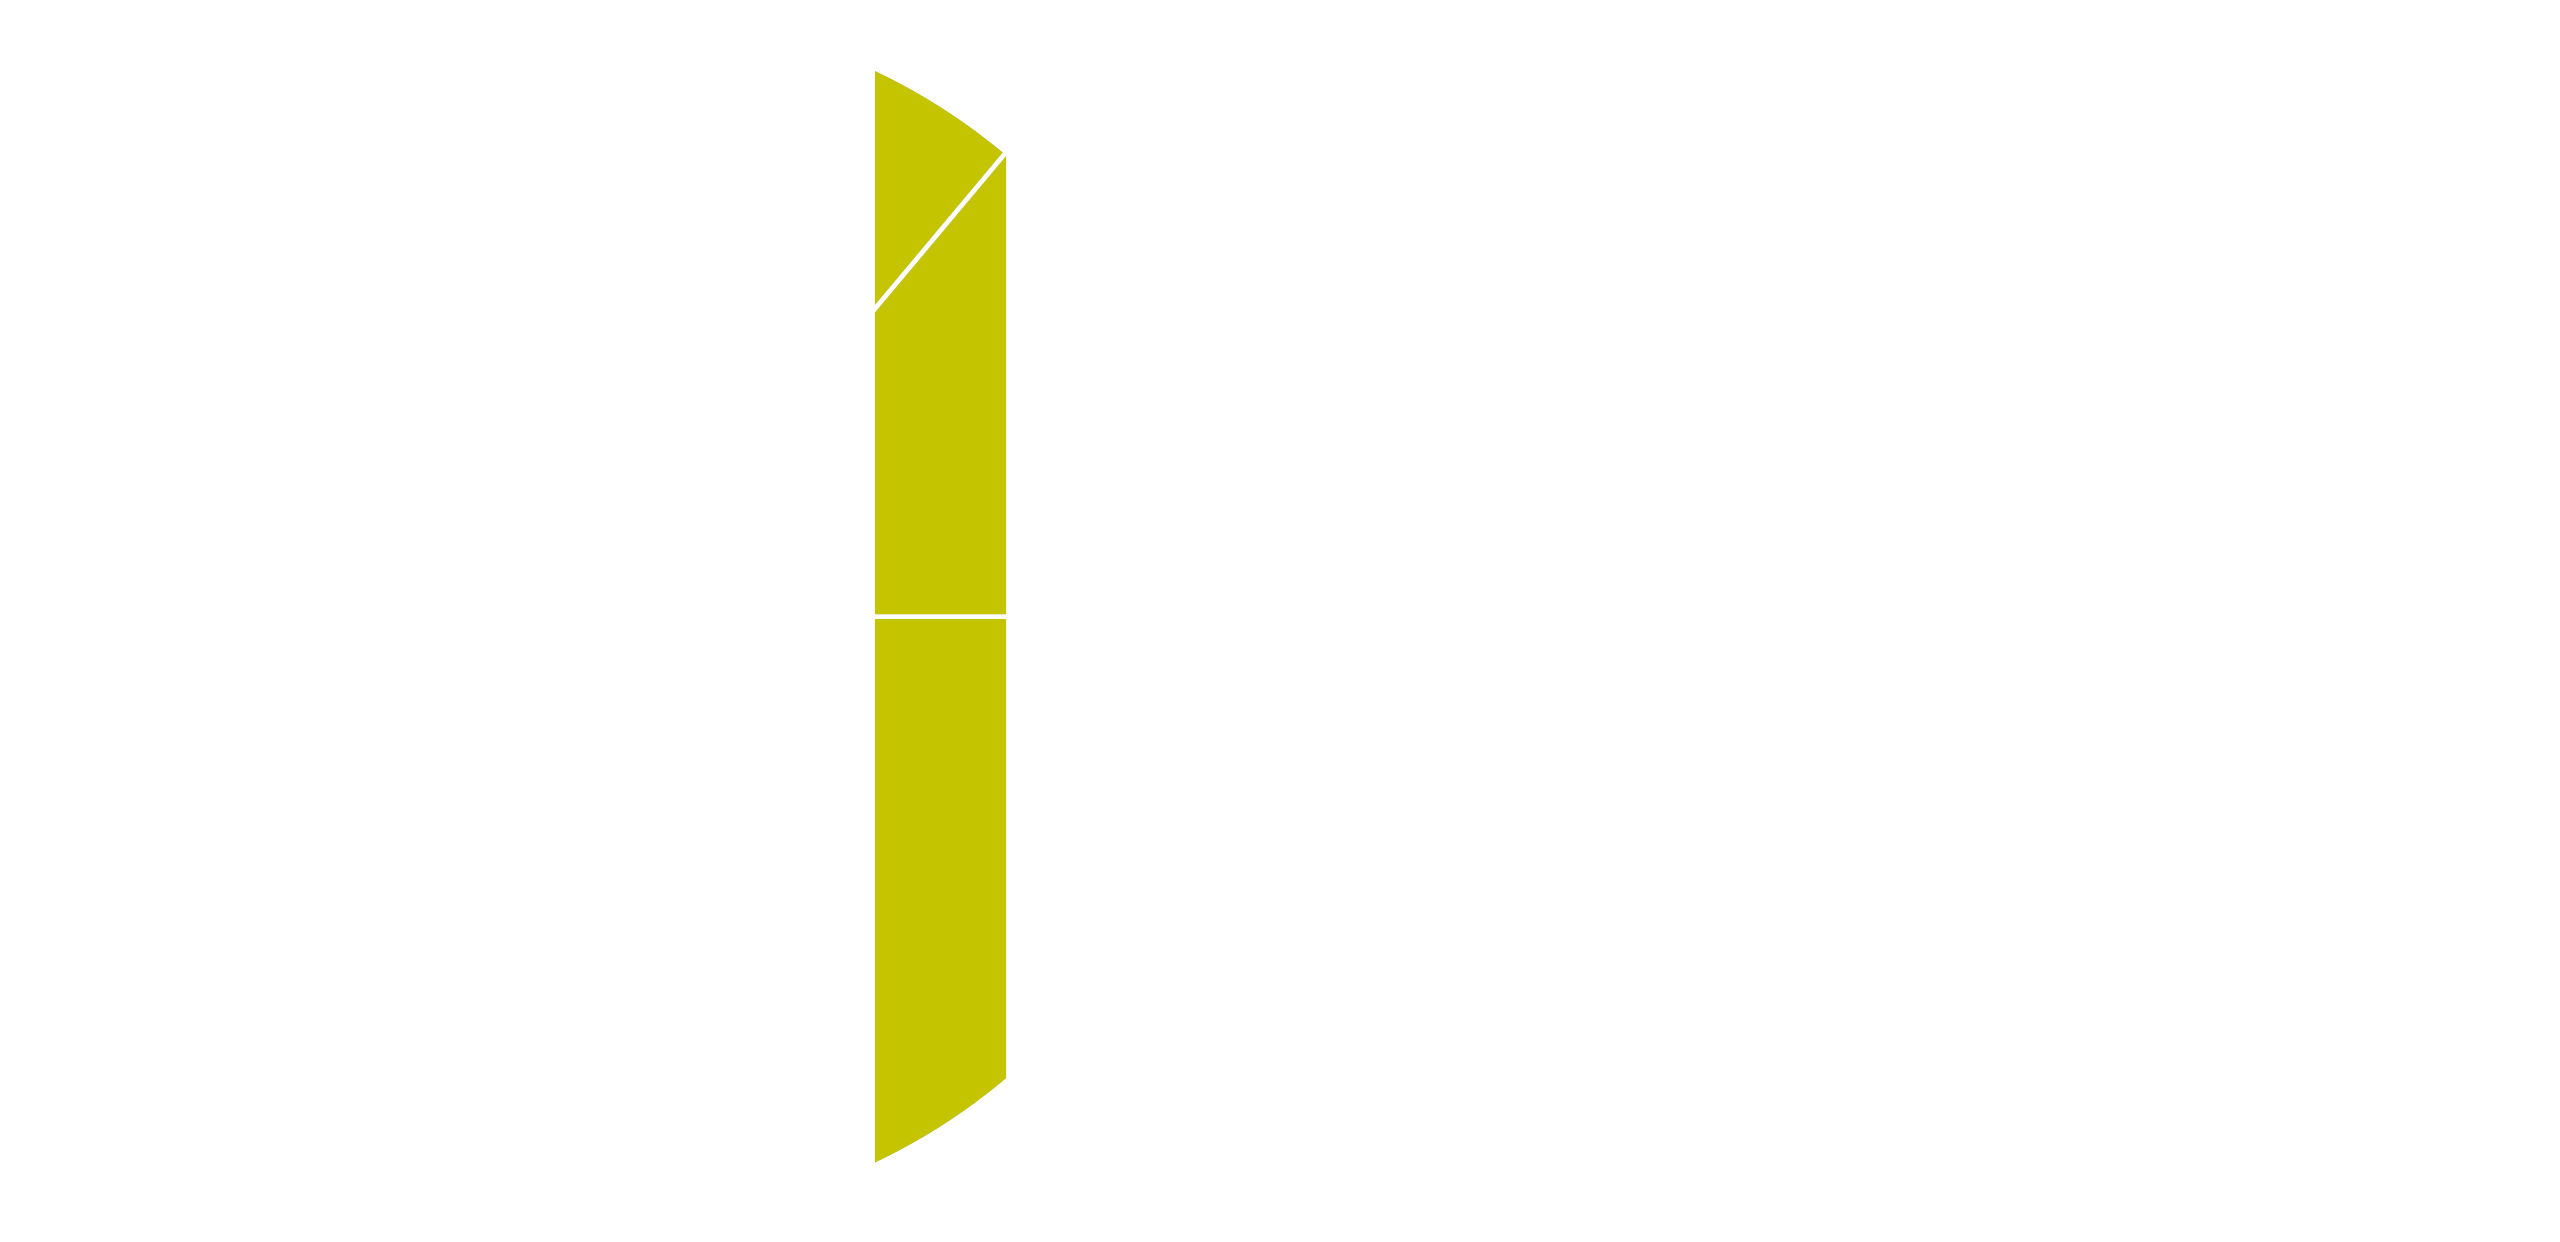
\includegraphics[width=0.99\textwidth]{Figures/Gravity/Exported/Shell-diag_reversed_CCBYSA4_0_Xaonon.png}
  \tiny [Xaononl CC BY-SA 4.0]

  \small Newton's shell theorem solves the volume integral inside and outside spherical objects ($\rightarrow$ Ex.-Discussion)
\end{PointSix}

\end{frame}

\begin{frame}
\begin{PointSix}{Newton's Shell Theorem}
 \begin{itemize}
    \item The field outside a shell is the same as the one from an equivalent point mass
    \item The field inside a shell is zero. Everywhere.
 \end{itemize}
\end{PointSix}
\end{frame}

\begin{frame}
\begin{PointSix}{Other shapes}
 \begin{itemize}
    \item \small There are analytical solutions for other shapes (e.g., Nagy 1966 for Prism).
 \end{itemize}
 \begin{center}
    \begin{tikzpicture}[>=latex,scale=2]

        \pgfmathsetmacro{\x}{1}
        \pgfmathsetmacro{\y}{1}
        \pgfmathsetmacro{\z}{1.5}
        \path (0,0,\y) coordinate (A) (\x,0,\y) coordinate (B) (\x,0,0) coordinate (C) (0,0,0)
        coordinate (D) (0,\z,\y) coordinate (E) (\x,\z,\y) coordinate (F) (\x,\z,0) coordinate (G)
        (0,\z,0) coordinate (H);
        \draw [thick] (-2,1.8) -- (3,1.8);
        \draw (A)--(B)--(C)--(G)--(F)--(B) (A)--(E)--(F)--(G)--(H)--(E);
        \draw (A)--(D)--(C) (D)--(H);
        \node[yshift=-0.3cm] at (2,1.8) {\small Surface};
        \draw[thin,|<->|] ($(A)+(0,-4pt)$) -- node[below]{x}($(B)+(0,-4pt)$);
        \draw[thin,|<->|] ($(B)+(-45:4pt)$) -- node[below,sloped]{y}($(C)+(-45:4pt)$);
        \draw[thin,|<->|] ($(C)+(4pt,0)$) -- node[below,sloped]{z}($(G)+(4pt,0)$);

    \end{tikzpicture}
\end{center}
\end{PointSix}
\end{frame}


\begin{frame}
\begin{PointSix}{Numerical forward modelling ($\rightarrow$ Ex)}
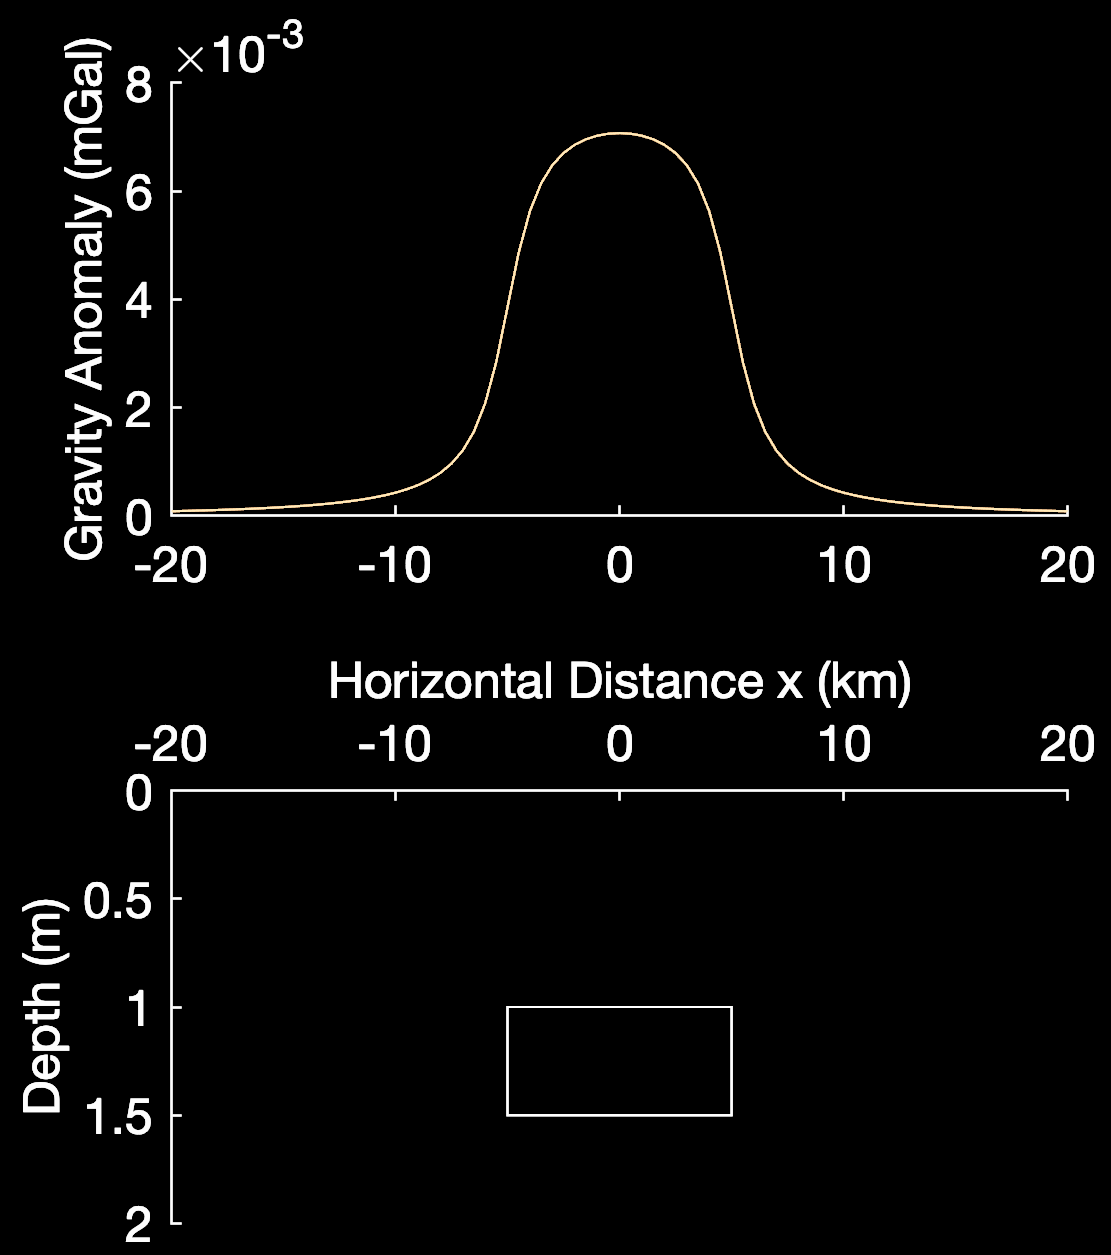
\includegraphics[width=0.8\textwidth]{Figures/Gravity/Exported/ForwardModelPrismReversed.png}
\end{PointSix}
\end{frame}



\begin{frame}
  \begin{PointSix}{Vector fields}
    \centering
    $
    \vec{g} = G\frac{M}{r^2}\hat{r}
    $
    \begin{center}
    \scalebox{0.85}{
        \begin{tikzpicture}
          \begin{axis}[
              xmin = -4, xmax = 4,
              ymin = -4, ymax = 4,
              zmin = 0, zmax = 1,
              axis equal image,
              xtick distance = 20,
              ytick distance = 20,
              view = {0}{90},
              scale = 1.25,
            % title = {\bf Vector Field $F = [-y,x]$},
              height=7cm,
            % xlabel = {$x$},
            % ylabel = {$y$},
              colormap/viridis,
            % colorbar,
            % colorbar style = {
            %     ylabel = {Vector Length}
            % }
            hide x axis,
            hide y axis,
          ]
          \addplot3[
                  point meta = {sqrt(x^2+y^2)},
                  quiver = {
                      u = {-x/sqrt(x^2+y^2)^2},
                      v = {-y/sqrt(x^2+y^2)^2},
                      scale arrows = 0.7,
                  },
                  quiver/colored = {mapped color},
                  -stealth,
                  samples = 10,
                  domain = -4:4,
                  domain y = -4:4,
                  ] {0};
          \end{axis}
          \draw [fill=white] (3.4,3.4) circle (0.5cm);
        \end{tikzpicture}
    }
      \end{center}

  \end{PointSix}
 \end{frame}

 \begin{frame}
  \begin{PointSix}{Potential Field}
    \centering
    $
    \vec{g} = G\frac{M}{r^2}\hat{r}
    $
    \begin{center}
    \scalebox{0.85}{
        \begin{tikzpicture}
          \begin{axis}[
              xmin = -4, xmax = 4,
              ymin = -4, ymax = 4,
              zmin = 0, zmax = 1,
              axis equal image,
              xtick distance = 20,
              ytick distance = 20,
              view = {0}{90},
              scale = 1.25,
            % title = {\bf Vector Field $F = [-y,x]$},
              height=7cm,
            % xlabel = {$x$},
            % ylabel = {$y$},
              colormap/viridis,
            % colorbar,
            % colorbar style = {
            %     ylabel = {Vector Length}
            % }
            hide x axis,
            hide y axis,
          ]
          \addplot3[
                  point meta = {sqrt(x^2+y^2)},
                  quiver = {
                      u = {-x/sqrt(x^2+y^2)^2},
                      v = {-y/sqrt(x^2+y^2)^2},
                      scale arrows = 0.7,
                  },
                  quiver/colored = {mapped color},
                  -stealth,
                  samples = 10,
                  domain = -4:4,
                  domain y = -4:4,
                  ] {0};

              %For some reason gnuplot does not work.
              % \addplot3[contour gnuplot={number=50,labels=false, draw color=blue},thick,]
              % {
              %   abs(((1)/sqrt((x-2)^2+y^2) - (1)/sqrt((x+2)^2+y^2)))<4 ? ((1)/sqrt((x-2)^2+y^2) - (1)/sqrt((x+2)^2+y^2)) : NaN
              % };
          \end{axis}
          \draw [fill=white] (3.4,3.4) circle (0.5cm);
          \draw [dotted, thick] (3.4,3.4) circle (1.cm);
          \draw [dotted, thick] (3.4,3.4) circle (2.cm);
          \draw [dotted, thick] (3.4,3.4) circle (4.cm);
        \end{tikzpicture}
      }
      \end{center}

  \end{PointSix}
 \end{frame}

 \begin{frame}
  \begin{PointSix}{Potential Field}
    \centering
    \small What is the amount of work required?
    \begin{center}
    \scalebox{0.85}{
        \begin{tikzpicture}
          \begin{axis}[
              xmin = -4, xmax = 4,
              ymin = -4, ymax = 4,
              zmin = 0, zmax = 1,
              axis equal image,
              xtick distance = 20,
              ytick distance = 20,
              view = {0}{90},
              scale = 1.25,
            % title = {\bf Vector Field $F = [-y,x]$},
              height=7cm,
            % xlabel = {$x$},
            % ylabel = {$y$},
              colormap/viridis,
            % colorbar,
            % colorbar style = {
            %     ylabel = {Vector Length}
            % }
            hide x axis,
            hide y axis,
          ]
          \addplot3[
                  point meta = {sqrt(x^2+y^2)},
                  quiver = {
                      u = {-x/sqrt(x^2+y^2)^2},
                      v = {-y/sqrt(x^2+y^2)^2},
                      scale arrows = 0.7,
                  },
                  quiver/colored = {mapped color},
                  -stealth,
                  samples = 10,
                  domain = -4:4,
                  domain y = -4:4,
                  ] {0};

              %For some reason gnuplot does not work.
              % \addplot3[contour gnuplot={number=50,labels=false, draw color=blue},thick,]
              % {
              %   abs(((1)/sqrt((x-2)^2+y^2) - (1)/sqrt((x+2)^2+y^2)))<4 ? ((1)/sqrt((x-2)^2+y^2) - (1)/sqrt((x+2)^2+y^2)) : NaN
              % };
          \end{axis}
          \draw [fill=white] (3.4,3.4) circle (0.5cm);
          \draw [dotted, thick] (3.4,3.4) circle (1.cm);
          \draw [dotted, thick] (3.4,3.4) circle (2.cm);
          \draw [dotted, thick] (3.4,3.4) circle (4.cm);
          \draw[-latex,thick,Karminrot,->] (4.1,4.1) -- (6.2,6.2) node[midway,left,rotate=0] {$r$};
        \end{tikzpicture}
    }
      \end{center}

  \end{PointSix}
 \end{frame}


\begin{frame}
  \begin{PointSix}{Potential Fields}
    \begin{align*}
      U(r) &=& -\int_{\infty}^r \vec{g}d{\vec{r}} \\
           &=& -\int_{\infty}^r gd{r} \\
           &=& -GM\int_{\infty}^r \frac{1}{r^2}d{r} \\
           &=& -GM \left[ -\frac{1}{r}\right]_{\infty}^r \\
           &=& GM\frac{1}{r}
    \end{align*}
    Potential for a point mass.
  \end{PointSix}
\end{frame}

\begin{frame}
  \begin{PointSix}{Potential Fields}
    \begin{align*}
      \vec{g}(r) = -\nabla U(r)
    \end{align*}
    \small
    \begin{itemize}
      \item It is sometimes easier to calculate the potential of an anomaly and to infer the acceleration via the gradient.
      \item Equipotential lines are perpendicular to the field direction.
      \item Equipotential lines are in general NOT lines of equal field strength (cf. with down-hill slope force in landscape)
    \end{itemize}
  \end{PointSix}
\end{frame}


\begin{frame}
\begin{PointSix}{Gravitational field of a spherical Earth}
  \small The Earth's rotation minimizes gravitational acceleration at the equator. At the poles it does nothing.
  \begin{center}
  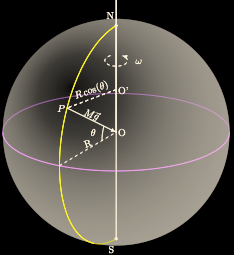
\includegraphics[width=0.6\textwidth]{Figures/Gravity/Exported/GravityFieldEarthRotation_Reversed.png}
  \end{center}
\end{PointSix}
\end{frame}




\begin{frame}
\begin{PointSix}{Gravitational field of a spherical Earth}
  \small Centripedal acceleration at P perpendicular to rotation axis parallel to O'-P:

  $$
  g_{r.} = \omega^2 R \cos(\theta)
  $$

  \small Centripedal acceleration at P perpendicular to rotation axis parallel to O'-P:

  $$
  g_{r.,proj.} = \omega^2 R \cos^2(\theta)
  $$

  \scalebox{0.6}{\parbox{\linewidth}{
    \begin{align*}
    &\text{Angular Frequency:}\, \omega \\
    &\text{Angular Velocity:}\, \vec{v}_r = \vec{\omega} \times \vec{R}\cos(\theta)\\
    &\text{Angular Acceleration:}\, \vec{g}_r = \dot{\vec{v}}_r=\vec{\omega} \times \vec{\omega} \times \vec{R}\cos(\theta)\\
    \end{align*}
  }}
\end{PointSix}
\end{frame}


\begin{frame}
\begin{PointSix}{An ellipsoidal Earth}
    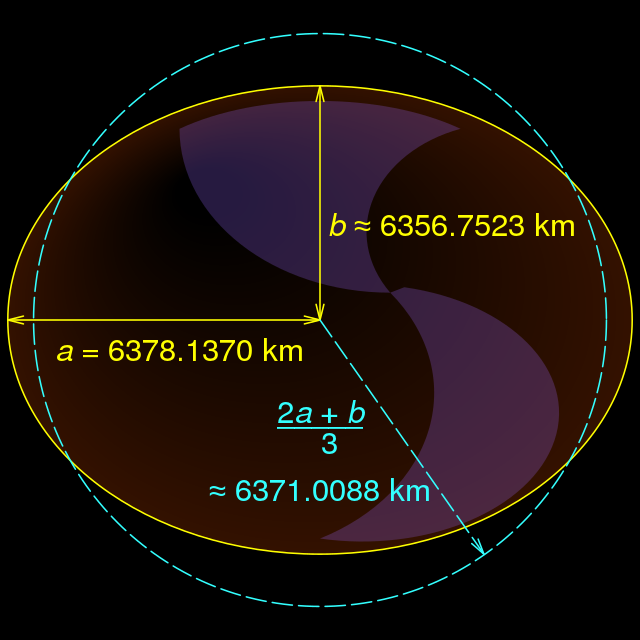
\includegraphics[width=0.8\textwidth]{Figures/Gravity/Exported/WGS84_mean_Earth_radius_Cmglee_Reversed.png}
    \tiny [Cmglee CCC 4.0]
\end{PointSix}
\end{frame}

\begin{frame}
\begin{PointSix}{Potential Fields}
  \begin{itemize}
    \item Rotation induces ellipsoidal shape approximate with reference ellipsoid.
    \item Latitudinal correction of gravitation is adjusted accordingly.
  \end{itemize}
\end{PointSix}
\end{frame}


\begin{frame}
  \begin{PointSix}{An ellipsoidal Earth}
      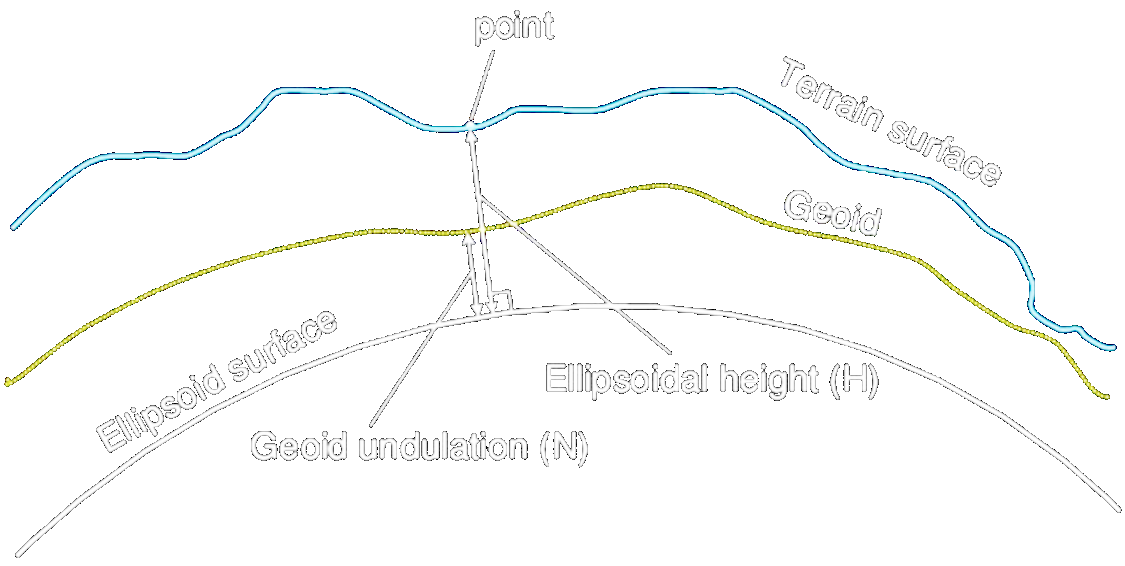
\includegraphics[width=0.9\textwidth]{Figures/Gravity/Exported/Geoid_Ziebart2004_TransparentBlack.png}

      \tiny [Ziebart et al., 2004] 

      \small
      \only<1>
      {
        \begin{itemize}
          \item Geoid is a real-world equipotential line approximating sea level.
          \item It is referenced to the geometric ellipsoid.
        \end{itemize}
      }
      \only<2>
      {
        \begin{itemize}
          \item 2 Geoid is a real-world equipotential line approximating sea level.
          \item 2 It is referenced to the geometric ellipsoid.
        \end{itemize}
      }
      \only<3>
      {
        \begin{itemize}
          \item Upwarping of geoid indicates mass excess.
          \item Downwarping of geoid indicates mass deficit.
        \end{itemize}
      }
  \end{PointSix}
  \end{frame}

%\begin{frame}
    \begin{PointSix}{Learning Goals}
      \alert{Learning goals today:}
      \begin{itemize}
        \item Principles of gravimeters.
        \item Gravity survey types (absolute \& relative) and general considerations of survey layouts and structure types.
        \item Reduction of gravity data.
      \end{itemize}
    \end{PointSix}
\end{frame}
  
\begin{frame}
    \begin{PointSix}{Spring-based gravimeters}
        \tiny [cc Reyko, CC-BY-SA3.0]
      \begin{center}
        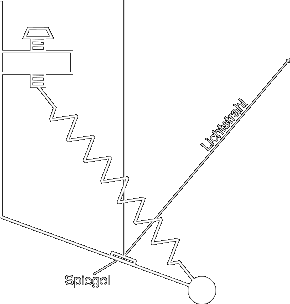
\includegraphics[width=0.6\textwidth]{Figures/Gravity/Exported/Reyko_CCBY-SA_LaCoste-Romberg_Reversed.png}
      
        \small Springconstant \& Extension.
      \end{center}
    \end{PointSix}
\end{frame}


\begin{frame}
  \begin{PointSix}{Pendulum-based gravimeters}
    
    \begin{center}
      \begin{tikzpicture}[font=\footnotesize]
        % Support
        \fill (-1.5,0) rectangle(1.5,0.1);

        % Bob's trajectory
        \draw[dashed] (-60:4) arc(-60:-120:4);

        % Rod + Bob
        \draw (0,0) -- (-60:4) node[fill,circle](m){};

        % Weight Force
        \draw[-latex] (m) -- node[right]{$\vec{g}$}++(0,-1) ;

        % Tension Force
        %\draw [-latex] (m) -- node[right]{$\vec{T}$}(-60:3);

        % Light gray pendulum
        \draw[black!10] (0,0) -- (-90:4) node[fill,circle]{};
        \draw[black!10] (0,0) -- (-120:4) node[fill,circle]{};
        \draw[<->,Karminrot] (0,0) -- (-90:4) node[midway,right]{l};
      \end{tikzpicture}

      Eigenfrequency \& Length.
      $$
      \omega = \sqrt{\frac{g}{l}}
      $$
    \end{center}
  \end{PointSix}
\end{frame}

\begin{frame}
  \begin{PointSix}{Free-fall gravimeters ($\rightarrow$ Ex.)}
      \tiny [FG Gravimeter from MicroGLaCoste]
    \begin{center}
      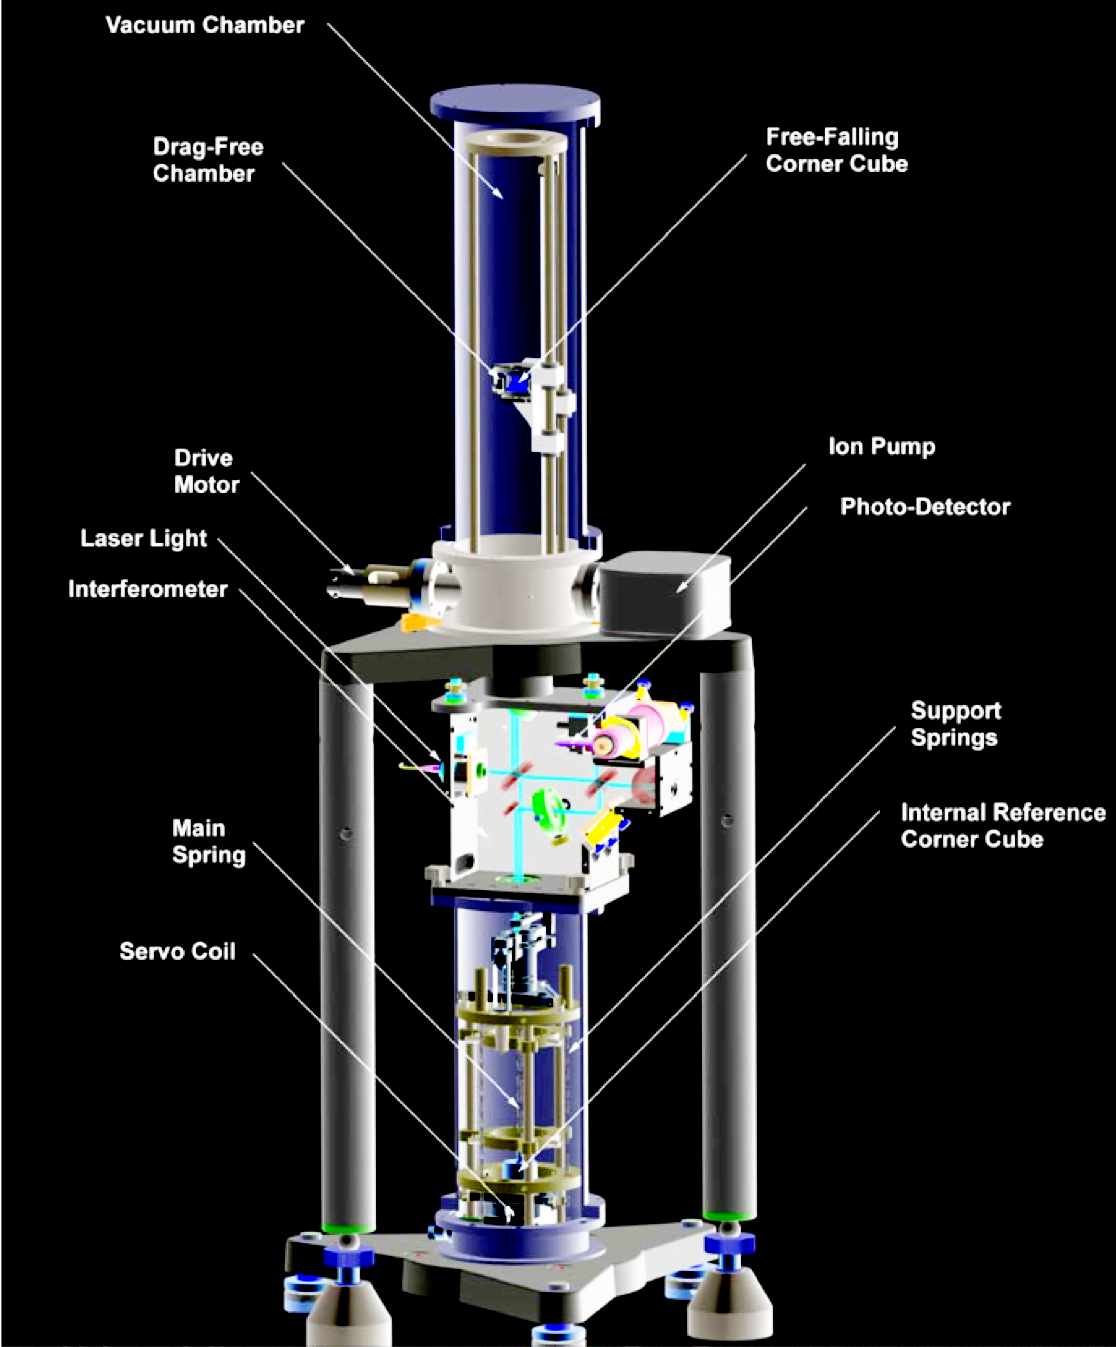
\includegraphics[width=0.55\textwidth]{Figures/Gravity/Exported/FG_Gravimeter_MicroGLaCoste_Reversed.png}

      \small Traveltime \& Distance.
    \end{center}
  \end{PointSix}
\end{frame}

\begin{frame}
  \begin{PointSix}{Gravimeters}
    \begin{itemize}
      \item Unit used is \textit{Gal} (=0.01 ms$^{-2}$)
      \item Top \textit{absolute} gravimeters $\sim 1 \mu$Gal ($10^{-9} g$)
      \item Top \textit{relative} gravimeters $\sim 10 \mu$Gal ($10^{-9} g$)
      \item Typically only $g_z$ is measured.
    \end{itemize}
  \end{PointSix}
\end{frame}
\begin{frame}
    \begin{PointSix}{Instrument drift / temporal variability}
      \resizebox{9 cm}{!}{     
              \begin{tikzpicture}[background rectangle/.style={fill=black},show background rectangle]
                \coordinate (TL) at (-2,-3);
                \coordinate (TR) at (9,-3);
                \coordinate (BL) at (-2,-10);
                \coordinate (BR) at (9,-10);
                \coordinate (Target) at (3.5,-5);

     

                \draw [->,thick,white] (TL) -- (TR) node[circle,fill=Karminrot,pos=0]{A} node[circle,fill=Karminrot,pos=0.2]{B} node[circle,fill=Karminrot,pos=0.4]{C} node[circle,fill=Karminrot,pos=0.6]{D} node[circle,fill=Karminrot,pos=0.8]{E} node[circle,fill=Karminrot,pos=1.0]{F};
                \fill[Karminrot] (Target) circle (2.5ex);
                %\draw[ultra thick,MyBlue] (-1.4,1.3) circle (2.5ex);
                %\draw [<-,line width=1.25mm,MyBlue]  (TL) to[out=30,in=150] (TR);
                \begin{axis}[
                    ylabel={Gravity Anomaly},
                    xlabel={Horizontal Distance},
                    label style={font=\small},
                    axis lines=middle, xtick=\empty,ytick=\empty,
                    color=white,
                    width=12cm,
                    height=\axisdefaultheight,
                    at={(-0.18\linewidth,0)},
                    axis line style=ultra thick,
                    x label style={at={(axis description cs:0.91,-0.025)},anchor=north},
                    y label style={at={(axis description cs:0.91,0.9)},anchor=north}
                      ]
                    \addplot[domain=-80:80,samples=200,color=Karminrot,line width=1.0mm] {5/((25+x*x)^(0.5)*1000)+x/1000000+1/10000};
                    %\addplot[domain=-80:80,samples=200,color=MyBlue,line width=1.0mm,dashed] {5/((25+x*x)^(0.5)*1000)};
                    %\addplot[domain=-80:-70,samples=200,color=Karminrot,mark=-*,line width=1.0mm,dashed] {x*0.0+3/10000};
                  \end{axis}
              \end{tikzpicture}
      }
    \end{PointSix}
\end{frame}


\begin{frame}
  \begin{PointSix}{Instrument drift / temporal variability}
    \resizebox{9 cm}{!}{     
            \begin{tikzpicture}[background rectangle/.style={fill=black},show background rectangle]
              \coordinate (TL) at (-2,-3);
              \coordinate (TR) at (9,-3);
              \coordinate (BL) at (-2,-10);
              \coordinate (BR) at (9,-10);
              \coordinate (Target) at (3.5,-5);

   

              \draw [->,thick,white] (TL) -- (TR) node[circle,fill=Karminrot,pos=0]{A} node[circle,fill=Karminrot,pos=0.2]{B} node[circle,fill=Karminrot,pos=0.4]{C} node[circle,fill=Karminrot,pos=0.6]{D} node[circle,fill=Karminrot,pos=0.8]{E} node[circle,fill=Karminrot,pos=1.0]{F};
              \fill[Karminrot] (Target) circle (2.5ex);
              \draw[ultra thick,MyBlue] (-1.4,1.3) circle (2.5ex);
              \node[MyBlue] at (-1.4,2.4) {offset};
              \draw [<-,line width=1.25mm,MyBlue]  (TL) to[out=30,in=150] (TR);
              \begin{axis}[
                  ylabel={Gravity Anomaly},
                  xlabel={Horizontal Distance},
                  label style={font=\small},
                  axis lines=middle, xtick=\empty,ytick=\empty,
                  color=white,
                  width=12cm,
                  height=\axisdefaultheight,
                  at={(-0.18\linewidth,0)},
                  axis line style=ultra thick,
                  x label style={at={(axis description cs:0.91,-0.025)},anchor=north},
                  y label style={at={(axis description cs:0.91,0.9)},anchor=north}
                    ]
                  \addplot[domain=-80:80,samples=200,color=Karminrot,line width=1.0mm] {5/((25+x*x)^(0.5)*1000)+x/1000000+1/10000};
                  \addplot[domain=-80:80,samples=200,color=MyBlue,line width=1.0mm,dashed] {5/((25+x*x)^(0.5)*1000)};
                  \addplot[domain=-80:-70,samples=200,color=Karminrot,mark=-*,line width=1.0mm,dashed] {x*0.0+3/10000};
                \end{axis}
            \end{tikzpicture}
    }
  \end{PointSix}
\end{frame}

\begin{frame}
  \begin{PointSix}{Absolute vs. relative}
    Absolute gravimeters are needed
    \begin{itemize}
      \item if loop closure if impossible (e.g. intercontinental surveys),
      \item for long-term changes such as isostatic uplift,
      \item as basestations for relative surveys.
    \end{itemize}
    Relative surveys are always easier to conduct and loop closure can cancel many error sources (e.g., instrument drift).
  \end{PointSix}
\end{frame}

\begin{frame}
  \begin{PointSix}{Reduction of gravity data}
    Every gravity survey measures:
    \begin{itemize}
      \item latitudinal variability,
      \item dependency on elevation,
      \item the surrounding terrain,
      \item excess mass above anomaly,
      \item earth \& ocean tides,
      \item (instr. drift, motion compons.).
      \item \alert{density variability in the subsurface.}
    \end{itemize}
  \end{PointSix}
\end{frame}

\begin{frame}
  \begin{PointSix}{Latitudinal variability ($\rightarrow$ Ex.)}
    \small  Extension to ellipsoid contains the same physics.
    \begin{center}
    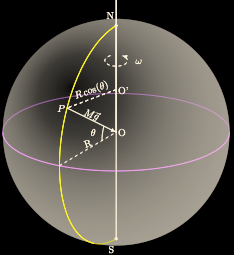
\includegraphics[width=0.5\textwidth]{Figures/Gravity/Exported/GravityFieldEarthRotation_Reversed.png}
    \end{center}
    \small Max 5 Gal (this is large!).
  \end{PointSix}
\end{frame}

\begin{frame}
  \begin{PointSix}{Reduction of gravity data}
    Every gravity survey measures:
    \begin{itemize}
      \item \textcolor{MyBlue}{latitudinal variability},
      \item dependency on elevation,
      \item the surrounding terrain,
      \item excess mass above anomaly,
      \item earth \& ocean tides,
      \item (instr. drift, motion compons.).
      \item \alert{density variability in the subsurface.}
    \end{itemize}
  \end{PointSix}
\end{frame}

\begin{frame}
  \begin{PointSix}{Elevation correction (i.e. free-air)}
    \resizebox{9 cm}{!}{     
            \begin{tikzpicture}[background rectangle/.style={fill=black},show background rectangle]
              \coordinate (TL) at (-2,-3);
              \coordinate (TR) at (9,-3);
              \coordinate (BL) at (-2,-10);
              \coordinate (BR) at (9,-10);
              \coordinate (Target) at (3.5,-5);

   

              \draw [->,thick,white] (TL) -- (TR) node[circle,fill=Karminrot,pos=0]{A} node[circle,fill=Karminrot,pos=0.2]{B} node[circle,fill=Karminrot,pos=0.4]{C} node[circle,fill=Karminrot,pos=0.6]{D} node[circle,fill=Karminrot,pos=0.8]{E} node[circle,fill=Karminrot,pos=1.0]{F};
              \fill[Karminrot] (Target) circle (2.5ex);
              \begin{axis}[
                  ylabel={Gravity Anomaly},
                  xlabel={Horizontal Distance},
                  label style={font=\small},
                  axis lines=middle, xtick=\empty,ytick=\empty,
                  color=white,
                  width=12cm,
                  height=\axisdefaultheight,
                  at={(-0.18\linewidth,0)},
                  axis line style=ultra thick,
                  x label style={at={(axis description cs:0.91,-0.025)},anchor=north},
                  y label style={at={(axis description cs:0.91,0.9)},anchor=north}
                    ]
                 % \addplot[domain=-80:80,samples=200,color=Karminrot,line width=1.0mm] {5/((25+x*x)^(0.5)*1000)+x/1000000+1/10000};
                  \addplot[domain=-80:80,samples=200,color=MyBlue,line width=1.0mm] {5/((25+x*x)^(0.5)*1000)};
                  %\addplot[domain=-80:-70,samples=200,color=Karminrot,mark=-*,line width=1.0mm,dashed] {x*0.0+3/10000};
                \end{axis}
            \end{tikzpicture}
    }
  \end{PointSix}
\end{frame}

\begin{frame}
  \begin{PointSix}{Elevation correction (i.e. free-air)}
    \resizebox{9 cm}{!}{     
            \begin{tikzpicture}[background rectangle/.style={fill=black},show background rectangle]
              \coordinate (TL) at (-2,-2);
              \coordinate (TR) at (9,-2);
              \coordinate (BL) at (-2,-10);
              \coordinate (BR) at (9,-10);
              \coordinate (Target) at (3.5,-5);

   

              \draw [->,thick,white] (TL) -- (TR) node[circle,fill=Karminrot,pos=0]{A} node[circle,fill=Karminrot,pos=0.2]{B} node[circle,fill=Karminrot,pos=0.4]{C} node[circle,fill=Karminrot,pos=0.6]{D} node[circle,fill=Karminrot,pos=0.8]{E} node[circle,fill=Karminrot,pos=1.0]{F};
              \fill[Karminrot] (Target) circle (2.5ex);
              \begin{axis}[
                  ylabel={Gravity Anomaly},
                  xlabel={Horizontal Distance},
                  label style={font=\small},
                  axis lines=middle, xtick=\empty,ytick=\empty,
                  color=white,
                  width=12cm,
                  height=\axisdefaultheight,
                  at={(-0.18\linewidth,0)},
                  axis line style=ultra thick,
                  x label style={at={(axis description cs:0.91,-0.025)},anchor=north},
                  y label style={at={(axis description cs:0.91,0.9)},anchor=north}
                    ]
                 % \addplot[domain=-80:80,samples=200,color=Karminrot,line width=1.0mm] {5/((25+x*x)^(0.5)*1000)+x/1000000+1/10000};
                 \addplot[domain=-80:80,samples=200,color=MyBlue,line width=1.0mm,dashed] {5/((25+x*x)^(0.5)*1000)};
                  \addplot[domain=-80:80,samples=200,color=MyBlue,line width=1.0mm] {0.6*5/((25+x*x)^(0.5)*1000)};
                  %\addplot[domain=-80:-70,samples=200,color=Karminrot,mark=-*,line width=1.0mm,dashed] {x*0.0+3/10000};
                \end{axis}
            \end{tikzpicture}
    }
  \end{PointSix}
\end{frame}

\begin{frame}
  \begin{PointSix}{Elevation correction}
    The elevation correction references the gravity anomaly to the same datum (e.g., the geoid). 
    
    \alert{How does the gravitational acceleration change with elevation near the Earth's surface?}
  \end{PointSix}
\end{frame}

\begin{frame}
  \begin{PointSix}{Elevation correction via Taylor expansion}
    Taylor expansion near $r=R_E$:
    \only<1>
    {
      $$
        g(r) = g(R_E) + \frac{dg}{dr}|_{R_E}
      $$
    }
    \only<2>
    {
      $$
        g(r) \approx G\frac{M}{R_E^2} - 2G\frac{M}{R_E^3}(r-R_E) + ...
      $$
    }
    \only<3>
    {
      $$
        g(r) \approx \underbrace{G\frac{M}{R_E^2}}_{\text{g at Earth's surface}} - 2G\frac{M}{R_E^3}(r-R_E) + ...
      $$
    }
    \only<4>
    {
      $$
        g(r) \approx G\frac{M}{R_E^2} - \underbrace{2G\frac{M}{R_E^3}(r-R_E)}_{\text{change with elevation}} + ...
      $$
    }
    \only<5>
    {
      $$
        g(r) \approx G\frac{M}{R_E^2} - \underbrace{2G\frac{M}{R_E^3}(r-R_E)}_{\text{change with elevation}} + ...
      $$
      Evaluation at let's say $r=R_E+1$ (m) returns a change of $\delta g(r)\approx -0.3$ mGal per m.
    }
    \only<6>
    {
      $$
        g(r) \approx G\frac{M}{R_E^2} - \underbrace{2G\frac{M}{R_E^3}(r-R_E)}_{\text{change with elevation}} + ...
      $$
      $\delta g(r)\approx -0.3$ mGal per m is large compared to the sensitivity of gravimeters, \alert{therefore the gravimeter elevation needs to be determined within centimeters using GNSS.}
    }
  \end{PointSix}
\end{frame}

\begin{frame}
  \begin{PointSix}{Reduction of gravity data}
    Every gravity survey measures:
    \begin{itemize}
      \item \textcolor{MyBlue}{latitudinal variability},
      \item \textcolor{MyBlue}{dependency on elevation},
      \item the surrounding terrain,
      \item excess mass above anomaly,
      \item earth \& ocean tides,
      \item (instr. drift, motion compons.).
      \item \alert{density variability in the subsurface.}
    \end{itemize}
  \end{PointSix}
\end{frame}

\begin{frame}
  \begin{PointSix}{Reduction of gravity data: Terrain correction}
   \begin{tikzpicture}
      \coordinate (TL) at (-2,-2);
      \coordinate (TR) at (9,-2);
      \coordinate (BL) at (-2,-10);
      \coordinate (BR) at (9,-10);
      \coordinate (Target) at (3.5,-3);

      \draw [->,thick,white] ([xshift=4cm,yshift=2cm] TL) -- ([yshift=2cm] TR);
      %\draw [->,thick,white,dashed] (TL) -- (TR) node[draw=none,fill=none,font=\scriptsize,near start,below] {reference surface};
      %\draw ([yshift=2cm] TL) .. controls ([xshift=2cm,yshift=4cm] TL) .. ([xshift=4.0cm,yshift=2cm] TL) ;
      \draw ([yshift=2cm] TL) ([xshift=4.0cm,yshift=2cm] TL) ;
      \fill[Karminrot] (Target) circle (2.5ex);
      %\draw [->, line width=1.5mm](3.5,0) -- (2.7,-1.7);
      \draw [->, line width=1.5mm,dashed](3.5,0) -- (3.5,-2);
     %\draw [line width=1.0mm,dashed](2.7,-1.7) -- (0,1) node[draw=none,fill=none,font=\small,midway,below,rotate=-46] {mass excess};
   \end{tikzpicture}
  \end{PointSix}
\end{frame}


\begin{frame}
  \begin{PointSix}{Reduction of gravity data: Terrain correction}
   \begin{tikzpicture}
      \coordinate (TL) at (-2,-2);
      \coordinate (TR) at (9,-2);
      \coordinate (BL) at (-2,-10);
      \coordinate (BR) at (9,-10);
      \coordinate (Target) at (3.5,-3);

      \draw [->,thick,white] ([xshift=4cm,yshift=2cm] TL) -- ([yshift=2cm] TR);
      %\draw [->,thick,white,dashed] (TL) -- (TR) node[draw=none,fill=none,font=\scriptsize,near start,below] {reference surface};
      \draw ([yshift=2cm] TL) .. controls ([xshift=2cm,yshift=4cm] TL) .. ([xshift=4.0cm,yshift=2cm] TL) ;
      \fill[Karminrot] (Target) circle (2.5ex);
      \draw [->, line width=1.5mm](3.5,0) -- (2.7,-2);
      \draw [->, line width=1.5mm,dashed](3.5,0) -- (3.5,-2);
      \draw [line width=1.0mm,dashed](2.7,-2) -- (0,1) node[draw=none,fill=none,font=\small,midway,below,rotate=-46] {mass excess};
   \end{tikzpicture}
  A neighboring mountain will reduce the measured $g_z$ independent of target properties.
  \end{PointSix}
\end{frame}
\begin{frame}
  \begin{PointSix}{Reduction of gravity data: Terrain correction}
   \begin{tikzpicture}
      \coordinate (TL) at (-2,-2);
      \coordinate (TR) at (9,-2);
      \coordinate (BL) at (-2,-10);
      \coordinate (BR) at (9,-10);
      \coordinate (Target) at (3.5,-3);

      \draw [->,thick,white] ([xshift=4cm,yshift=2cm] TL) -- ([yshift=2cm] TR);
      %\draw [->,thick,white,dashed] (TL) -- (TR) node[draw=none,fill=none,font=\scriptsize,near start,below] {reference surface};
      \draw ([yshift=2cm] TL) .. controls ([xshift=2cm,yshift=0cm] TL) .. ([xshift=4.0cm,yshift=2cm] TL) ;
      \fill[Karminrot] (Target) circle (2.5ex);
      \draw [->, line width=1.5mm](3.5,0) -- (4.3,-2);
      \draw [->, line width=1.5mm,dashed](3.5,0) -- (3.5,-2);
      \draw [line width=1.0mm,dashed](3.5,-2) -- (0,-1) node[draw=none,fill=none,font=\small,midway,below,rotate=-20] {mass deficit};
   \end{tikzpicture}
  A neighboring valley will reduce the measured $g_z$ independent of target properties.
  \end{PointSix}
\end{frame}

\begin{frame}
  \begin{PointSix}{Reduction of gravity data: Terrain correction}
  \begin{itemize}
    \item The terrain correction requires an elevation model and assumptions about the broad-scale sub-surface density.
    \item The terrain correction is positive both for surrounding valleys and mountains.
  \end{itemize}
\end{PointSix}
\end{frame}

\begin{frame}
  \begin{PointSix}{Reduction of gravity data}
    Every gravity survey measures:
    \begin{itemize}
      \item \textcolor{MyBlue}{latitudinal variability},
      \item \textcolor{MyBlue}{dependency on elevation},
      \item \textcolor{MyBlue}{the surrounding terrain},
      \item excess mass above anomaly,
      \item earth \& ocean tides,
      \item (instr. drift, motion compons.).
      \item \alert{density variability in the subsurface.}
    \end{itemize}
  \end{PointSix}
\end{frame}

\begin{frame}
  \begin{PointSix}{Reduction of gravity data: Terrain correction}
   \begin{tikzpicture}
      \coordinate (TL) at (-2,-2);
      \coordinate (TR) at (9,-2);
      \coordinate (BL) at (-2,-10);
      \coordinate (BR) at (9,-10);
      \coordinate (Target) at (3.5,-3);

      \draw [->,thick,white] ([xshift=4cm,yshift=2cm] TL) -- ([yshift=2cm] TR);
      \draw [->,thick,white,dashed] (TL) -- (TR) node[draw=none,fill=none,font=\scriptsize,near start,below] {reference surface};
      \draw ([yshift=2cm] TL) .. controls ([xshift=2cm,yshift=4cm] TL) .. ([xshift=4.0cm,yshift=2cm] TL) ;
      \fill[Karminrot] (Target) circle (2.5ex);
      \draw [->, line width=1.5mm,Karminrot](3.5,0) -- (3.5,-1);

   \end{tikzpicture}
  \small Elevation and terrain correction to not account for the mass between the measurement surface and the reference surface.
  \end{PointSix}
\end{frame}

\begin{frame}
  \begin{PointSix}{Reduction of gravity data: Terrain correction}
   \begin{tikzpicture}
      \coordinate (TL) at (-2,-2);
      \coordinate (TR) at (9,-2);
      \coordinate (BL) at (-2,-10);
      \coordinate (BR) at (9,-10);
      \coordinate (Target) at (3.5,-3);

      %\draw [->,thick,white] ([xshift=4cm,yshift=2cm] TL) -- ([yshift=2cm] TR);
      %\draw [->,thick,green,name path = A] ([yshift=2cm] TL) -- ([yshift=2cm] TR);
      \draw [->,thick,white,dashed,name path = B] (TL) -- (TR) node[draw=none,fill=none,font=\scriptsize,near start,below] {reference surface};
      \draw ([yshift=2cm] TL) .. controls ([xshift=2cm,yshift=4cm] TL) .. ([xshift=4.0cm,yshift=2cm] TL) ;
      \fill[Karminrot] (Target) circle (2.5ex);
      \fill[pattern=north west lines,pattern color=white] ([yshift=2cm] TL) rectangle (TR);
      \draw [->, line width=1.5mm,Karminrot](3.5,0) -- (3.5,-1);
      \draw [|-|, line width=0.5mm,white]([xshift=-0.5cm] TL) -- ([xshift=-0.5cm, yshift=2cm] TL) node[draw=none,fill=none,font=\scriptsize,midway,left] {h};;
      
   \end{tikzpicture}
  \only<1>{
    \small What is the effect $\delta g_z$ of a horizontal plate with constant density?
  }
  \only<2>{
    \small $g_z = G \rho \int \int \int \frac{1}{r^2}\cos(\phi) dV = ? $
  }
  \only<3>{
    \small $g_z = G \rho \int \int \int \frac{1}{r^2}\cos(\phi) dV = 2\pi G\rho h$
  }
  \end{PointSix}
\end{frame}
\begin{frame}
  \begin{PointSix}{Reduction of gravity data}
    Every gravity survey measures:
    \begin{itemize}
      \item \textcolor{MyBlue}{latitudinal variability},
      \item \textcolor{MyBlue}{dependency on elevation},
      \item \textcolor{MyBlue}{the surrounding terrain},
      \item \textcolor{MyBlue}{excess mass above anomaly},
      \item earth \& ocean tides,
      \item (instr. drift, motion compensation),
      \item \alert{density variability in the subsurface.}
    \end{itemize}
  \end{PointSix}
\end{frame}

\begin{frame}
  \begin{PointSix}{The origin of tides}
      \begin{itemize}
        \item Tides are caused by gravity celestial bodies (i.e. Sun \& Moon).
        \item Tidal forces vary across a spatially extended body.
        \item Tidal forces are balanced by centrifugal forces of two (three) body rotations.
      \end{itemize}
  \end{PointSix}
\end{frame}

\begin{frame}
  \begin{PointSix}{The origin of tides}
  \begin{tikzpicture}
    \coordinate (EC) at (5,0) node[yshift=-2cm,draw=none,fill=none,font=\small,below] {Earth};
    \coordinate (MC) at (0,0) node[yshift=-2cm,xshift=5cm,draw=none,fill=none,font=\small,below] {Moon};
    \fill[white] (EC) circle (4.5ex);
    \fill[white] (MC) circle (1.5ex);
    %§\draw [->, line width=1.5mm,Karminrot](EC) -- (MC);
    % \begin{axis}[
    %   ylabel={F},
    %   xlabel={distance r},
    %   label style={font=\tiny},
    %   axis lines=middle, xtick=\empty,ytick=\empty,
    %   color=Karminrot,
    %   width=8cm,
    %   height=4cm,
    %   ymin=0.0,
    %   %ymax=5.16,
    %   at={(0.0\linewidth,0.0\linewidth)},
    %   axis line style=ultra thick,
    %   x label style={at={(axis description cs:0.4,-0.025)},anchor=north},
    %   y label style={at={(axis description cs:-0.1,0.9)},anchor=north}
    %     ]

    %  \addplot[domain=0.6:1.5,samples=200,color=MyBlue,line width=1.0mm,dashed] {1/(x*x))};
    % \end{axis}
  \end{tikzpicture}
  \end{PointSix}
\end{frame}

\begin{frame}
  \begin{PointSix}{The origin of tides}
  \begin{tikzpicture}
    \coordinate (EC) at (5,0) node[yshift=-2cm,draw=none,fill=none,font=\small,below] {Moon};
    \coordinate (MC) at (0,0) node[yshift=-2cm,xshift=5cm,draw=none,fill=none,font=\small,below] {Earth};
    \fill[white] (EC) circle (4.5ex);
    \fill[white] (MC) circle (1.5ex);
    %§\draw [->, line width=1.5mm,Karminrot](EC) -- (MC);
    \begin{axis}[
      ylabel={F},
      xlabel={distance r},
      label style={font=\tiny},
      axis lines=middle, xtick=\empty,ytick=\empty,
      color=Karminrot,
      width=8cm,
      height=4cm,
      ymin=0.0,
      %ymax=5.16,
      at={(0.0\linewidth,0.0\linewidth)},
      axis line style=ultra thick,
      x label style={at={(axis description cs:0.4,-0.025)},anchor=north},
      y label style={at={(axis description cs:-0.1,0.9)},anchor=north}
        ]

     \addplot[domain=0.6:1.5,samples=200,color=MyBlue,line width=1.0mm,dashed] {1/(x*x))};
    \end{axis}
  \end{tikzpicture}
  \vspace{1cm}

  \small Gravitational attraction is stronger on the nearside than the farside.
  \end{PointSix}
\end{frame}

\begin{frame}
  \begin{PointSix}{The origin of tides}
    \begin{tikzpicture}
        \coordinate (EC) at (5,0);
        \coordinate (MC) at (0,0);
        \coordinate (RP) at (4,0);
        \fill[white] (EC) circle (4.5ex) node[yshift=-2cm,draw=none,fill=none,font=\small,below] {Earth};
        \fill[white] (MC) circle (1.5ex) node[yshift=-2cm,draw=none,fill=none,font=\small,below] {Moon};
        \fill[Karminrot] (RP) circle (0.5ex);
        \draw [->,thick,Karminrot] (RP) -- ([yshift=2cm] RP) node [midway] {\AxisRotator[rotate=-90]};
        \draw [|-|,thick,Karminrot] (EC) -- (MC);
   \end{tikzpicture}
   
          \pause
          \small Centrifugal force can be projected into radial (i.e. parallel to Earth's gravitation) and parallel component. This leads to the force balance.
  \end{PointSix}
\end{frame}

\begin{frame}
  \begin{PointSix}{The origin of tides}
  \begin{tikzpicture}
    \coordinate (RP) at (1,0);
    \node[inner sep=0pt] (russell) at (0,0)
      {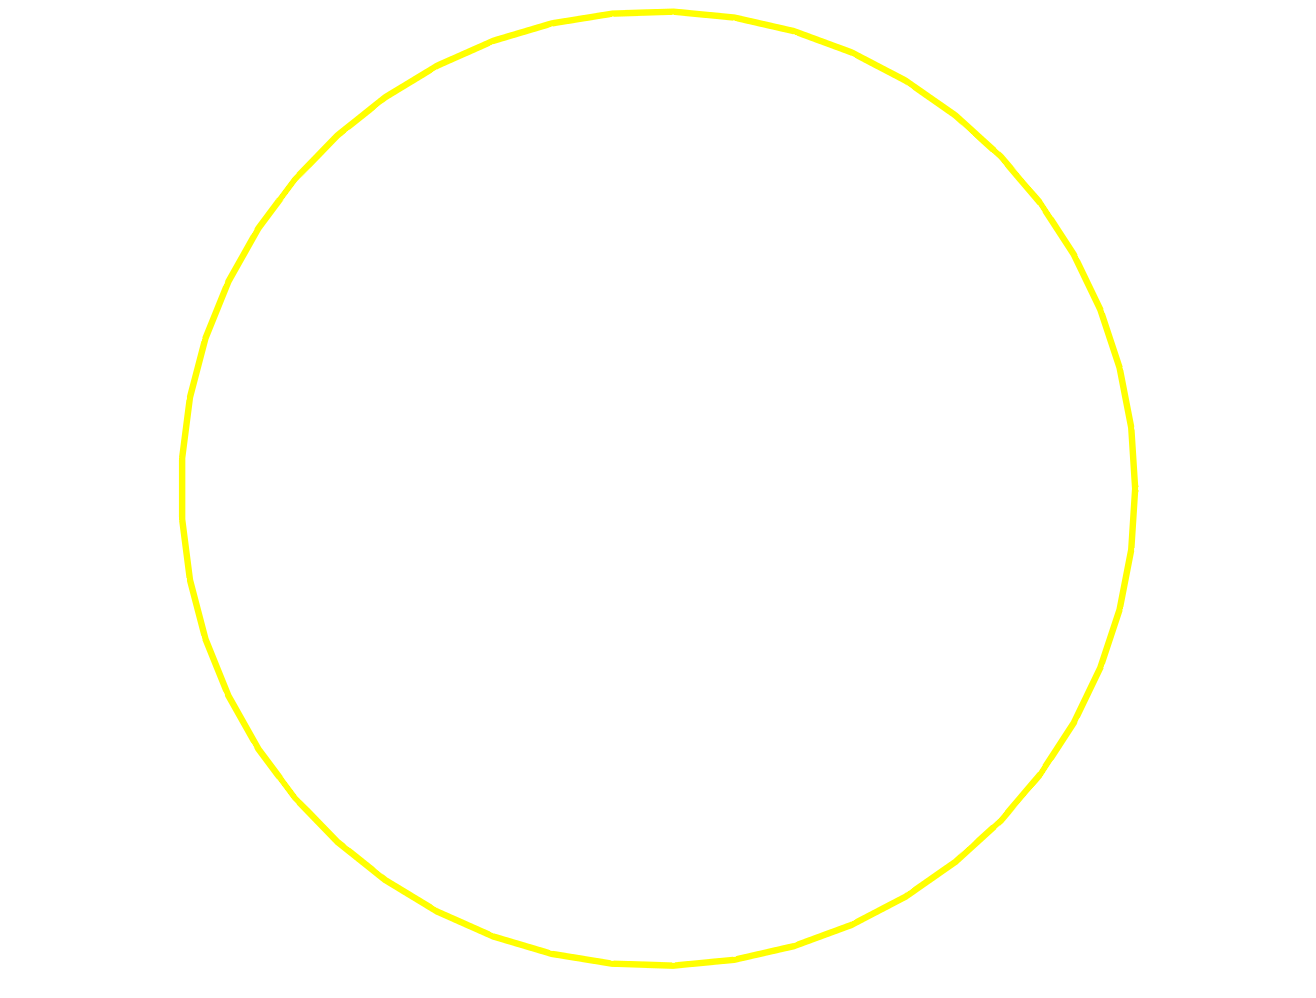
\includegraphics[width=.6\textwidth]{Figures/Gravity/Exported/Field_tidal.png}};
      \fill[white] (5,0) circle (1.5ex) node[yshift=-2cm,draw=none,fill=none,font=\small,below] {Moon};
      \draw [->,thick,Karminrot] (RP) -- ([yshift=2cm] RP) node [midway] {\AxisRotator[rotate=-90]};
      \draw [|-|,thick,Karminrot] (RP) -- (5,0);
  \end{tikzpicture}
  \small The lunar gravity differential field is responsible for two tidal bulges (i.e. tides twice a day).
\end{PointSix}
\end{frame}

\begin{frame}
  \begin{PointSix}{The origin of tides}
      \small
      \begin{itemize}
        \item Tidal forces vary across a spatially extended body.
        \item Tidal forces are balanced by centrifugal forces of two (three) body rotations.
        \item There is lots of confusion regarding the origin of tides (cf. Matsuda et al. 2015 $\rightarrow$ Ilias).
        \item \color{MyBlue}{Tide models can be used for correction} 
      \end{itemize}
  \end{PointSix}
\end{frame}

\begin{frame}
  \begin{PointSix}{Reduction of gravity data}
    Every gravity survey measures:
    \begin{itemize}
      \item \textcolor{MyBlue}{latitudinal variability},
      \item \textcolor{MyBlue}{dependency on elevation},
      \item \textcolor{MyBlue}{the surrounding terrain},
      \item \textcolor{MyBlue}{excess mass above anomaly},
      \item \textcolor{MyBlue}{earth \& ocean tides},
      \item (instr. drift, motion compensation),
      \item \alert{density variability in the subsurface.}
    \end{itemize}
  \end{PointSix}
\end{frame}

\begin{frame}
  \begin{PointSix}{Reduction of gravity data}
    Every gravity survey measures:
    \begin{itemize}
      \item \textcolor{MyBlue}{latitudinal variability},
      \item \textcolor{MyBlue}{dependency on elevation},
      \item \textcolor{MyBlue}{the surrounding terrain},
      \item \textcolor{MyBlue}{excess mass above anomaly},
      \item \textcolor{MyBlue}{earth \& ocean tides},
      \item \textcolor{MyBlue}{(instr. drift, motion compensation)},
      \item \alert{density variability in the subsurface.}
    \end{itemize}
  \end{PointSix}
\end{frame}



\end{document}​

